\documentclass[11pt,a4paper]{report}
\usepackage[utf8]{inputenc}
\usepackage[english]{babel}
\usepackage[T1]{fontenc}
\usepackage{amsmath}
\usepackage{amsfonts}
\usepackage{amssymb}
\usepackage{makeidx}
\usepackage{graphicx}
\usepackage{float}
\usepackage{lmodern}
\usepackage[dvipsnames]{xcolor}
\usepackage{tikz}
\usetikzlibrary{intersections}
\usepackage{pgfplots}
\usetikzlibrary{calc}
\usepackage{geometry}
\geometry{hmargin=2cm,vmargin=2cm}
\usepackage{fancybox}
\usepackage{mathtools}
\usepackage{enumitem}
\usepackage{tcolorbox}
\usepackage{colortbl}
\usepackage{fancybox}
\tcbuselibrary{most}
\usepackage{pifont}
\usepackage[skip = 2pt, font = footnotesize]{caption}
\usepackage{subcaption}
\usepackage{eso-pic}
\usepackage{nicematrix}
\usepackage{multicol}
\usepackage{booktabs}
\usepackage{svg}
\usepackage{derivative}
\usepackage{wrapfig}
\usepackage{stmaryrd}
\usepackage{yfonts}
\usepackage[backend=biber]{biblatex}
\addbibresource{references.bib}
\author{Andrea}
\setlength{\columnsep}{.5cm}
\renewcommand{\thesection}{\Roman{section}}
\renewcommand{\thesubsection}{\arabic{subsection}}
\renewcommand{\thesubsubsection}{\alph{subsubsection}}
\usepackage{amsmath}
\colorlet{shadecolor}{cyan!15}
\usepackage{fancyhdr}
\usepackage{etoolbox}
\usepackage[export]{adjustbox}
\usepackage{fourier-orns}
\usepackage{lettrine}
\usepackage{physics}
\definecolor{RoyalRed}{RGB}{157,16, 45}
\usepackage{titlesec}
\usepackage{lipsum} 
\titleclass{\chapter}{straight}
\titleformat{\chapter}[display]
{\normalfont\bfseries\filcenter}
{\color{black}\LARGE\thechapter}
{1ex}
{\color{black}\titlerule[2pt]
\vspace{2ex}%
\LARGE}
[\vspace{1ex}%
{\titlerule[2pt]}]

\usepackage[export]{adjustbox}
\renewcommand{\headrule}{%
\vspace{6pt}\hrulefill
\raisebox{0pt}{\quad\decofourleft\decotwo\decofourright\quad}\hrulefill}
\pagestyle{fancy}
\fancyhf{}
\rhead{ \textcolor{black}{\footnotesize \today}}
\lhead{ENS}
\chead{ \textcolor{black}{· \emph{Shallow Water Equations \& Poincarré Waves} ·}}
\rfoot{Andrea Combette}
\fancyfoot[C]{\thepage} 

\newlength{\tabcont}

\setlength{\parindent}{0.0in}
\setlength{\parskip}{0.05in}

\setcounter{tocdepth}{4}
\setcounter{secnumdepth}{4}

\begin{document}
\begin{titlepage}
    \AddToShipoutPictureBG*{
        \begin{tikzpicture}[overlay,remember picture]
            \draw [line width=3pt]
            ($ (current page.north west) + (2cm,-2.0cm) $)
            rectangle
            ($ (current page.south east) + (-2cm,1.8cm) $);
            \draw [line width=1pt]
            ($ (current page.north west) + (2.15cm,-2.15cm) $)
            rectangle
            ($ (current page.south east) + (-2.15cm,1.95cm) $);
        \end{tikzpicture}
    }
    \begin{center}
        \vspace*{2cm}
        \emph{\footnotesize{Department of physics, École Normale Supérieure, Paris}}

        \vspace*{1cm}

        \textsc{Shallow water equations and Poincarré waves}
        \vspace*{1cm}

        \rule{14cm}{2pt}\vspace{.7cm}

        \Large{\textbf{Report on Numerical Methods}}

        \vspace{.5cm}
        \rule{14cm}{2pt}
        \vspace{1cm}

        \Large Andrea Combette

        \vspace{3cm}

        \raisebox{-5pt}{\quad\decofourleft\decotwo\decofourright\quad}

        \vspace{6cm}

        \begin{minipage}{14cm}
            \small{
                \textbf{Cautionary note : } This paper is a report on numerical methods for the shallow water equations and gravity waves. It is not intended to be a complete and rigorous study of the subject. The reader is invited to refer to the references for further details.
                It has been made by a Master Student, with some background in physics and mathematics, but no prior knowledge of the subject. It is therefore not intended to be a reference for experts in the field.}
        \end{minipage}

    \end{center}

\end{titlepage}

\newpage
\tableofcontents
\newpage


\begin{center}
    \vspace*{1.5cm}\Large{\textbf{Abstract}}
    \vspace*{1cm}
    \fontsize{11}{18 }\selectfont

    \begin{minipage}{.7\linewidth}
        \lettrine[lines=4]{\color{black} S}{hallow} water equations, fundamental in fluid dynamics, offer a concise framework for studying the dynamics of a fluid layer with constant depth. They serve as a versatile tool to model various natural phenomena, including tsunami propagation, river flow, tidal patterns, and atmospheric behaviors. Derived from the more intricate Navier-Stokes equations, the shallow water equations assume a thin fluid layer compared to its horizontal extent, allowing the neglect of the vertical velocity component and approximating pressure as hydrostatic in the vertical direction. This simplification enables integration over the vertical dimension, facilitating a more tractable analysis.
        The primary focus of this report lies in the exploration of shallow water equations across diverse domains, with a specific emphasis on understanding the behavior of solutions, notably the emergence of Poincaré waves. Poincaré waves represent a specific subset of solutions characterized by their frictionless and Coriolis-dependent nature. Within this broader context, attention will be directed towards more specialized solutions, including Rossby, Kelvin, and gravity-Rossby mixed waves.
        These distinctive waves hold significant relevance in oceanography, where they play a pivotal role in the formation of oceanic currents, exemplified by the Gulf Stream. Additionally, they contribute to the genesis of the El Niño phenomenon, a climatic event with profound implications for Earth's climate. Delving deeper into the analysis, a specific subset of solutions within the Poincaré space emerges as solitons. These solitons, characterized by their lack of damping effects, serve as a valuable metric for evaluating the efficiency of numerical integration schemes. Notably, any observed damping effects in solitons can be attributed solely to numerical errors, making them a reliable benchmark for assessing the accuracy of the chosen numerical integration approach.\newpage
    \end{minipage}
\end{center}
\newpage
\fontsize{10}{10}\selectfont
\begin{multicols}{2}
    \chapter{Theoretical Background}
    \section{Shallow water equations}
    \lettrine[lines=2, lhang=.3, nindent=0pt]{\color{black} T}{he} shallow water equations considering small perturbations of speed and height regarding the mean field, and getting rid of the friction term is the following:
    \begin{equation*}
        \begin{cases}
            \partial_t u + U \partial_x u + V \partial_y u - fv = -g \partial_x h \\
            \partial_t v + U \partial_x v + V \partial_y v + fu = -g \partial_y h \\
            \partial_t h + U\partial_x (h) + V\partial_y (V) + a_0( \partial_x u + \partial_y v) = 0
        \end{cases}
    \end{equation*}

    With $U$ and $V$ the mean velocity in respective $x$ and $y$ direction verifying by the following equations:
    \begin{equation*}
        \begin{cases}
            u = U + u' \\
            v = V + v'
        \end{cases}
    \end{equation*}
    h is the height of the fluid perturbation, and $a_0$ is the mean depth of the fluid layer. $f$ is the Coriolis parameter given by $f = 2\Omega \sin (\theta)$, with $\Omega$ the rotation speed of earth and $\theta$ the co-latitude, finally $g$ is the gravity acceleration.
    In the following we will omit the prime notation for the perturbations of velocity.

    \begin{figure}[H]
        \def\svgwidth{1.2\linewidth}
        \input{./figure/height_def.pdf_tex}
        \caption{\footnotesize{Parametrisation of the fluid layer, as well as the height of the perturbation,
                note that $h$ is not define positive}}
        \label{fig:param}
    \end{figure}


    Then this give us in the reference frame of the wave propagation ($U,V$):
    \begin{equation} \label{eq:1}
        \begin{cases}
            \partial_t u  - fv = -g \partial_x h \\
            \partial_t v + fu = -g \partial_y h  \\
            \partial_t h + a_0( \partial_x u + \partial_y v) = 0
        \end{cases}
    \end{equation}
    Solutions of these equations are called Poincarré wave \cite{water}, these waves are dispersive since the phase speed $c_\Phi$ depends normally on the wave vector \textbf{k}.
    Nonetheless, these equations are not always easily linearized. Indeed, the Coriolis term is not constant on the domain of study, this brings some non-linearity in the equations. In the following we will study the behavior of these equations on different domains, and try to find some analytical solutions to them.
    Note that this non-linearity in \ref{eq:1} can be used to compensate the dispersion of the waves. Which will leads to \textbf{KDV} or \textbf{MKDV} equations when non-linearity $\sim$ dispersion, which are used to model one crest unimontane solitons \cite{Boyd80}. The case of high non-linearity wave is described by the \textbf{One dimensional advection equation}, in this case the phase velocity of the wave is constant.
    Finally, strong dispersive waves are described by the \textbf{NLS} equation.
    \section{Equatorial study}

    In this section we will study the behavior of the shallow water equations near the equator. This domain is of particular interest since the Coriolis term may be simplified to linearize the differential equations, to find analytical solutions to them.
    For example,  we can unearth some Kelvin wave solution, which are called Kelvin equatorial waves \cite{Holton}, deriving from coastal kelvin wave. These atmospheric waves can propagate eastward, with a given phase speed $c_\Phi^{Kelvin}$, though this wave type is non-dispersive due to high non-linearity, which leads to a constant phase speed $c_\phi^{Kelvin} = \sqrt{ga}$. Furthermore, another type of solution can be found, these are called equatorial Rossby waves and propagate westward with a phase speed $c_\Phi^{Rossby}$. We will see Rossby waves can be weakly or strongly dispersive depending on their size (i.e. on the \textbf{zonal wave number})

    \begin{figure}[H]
        \hspace*{-3.8cm}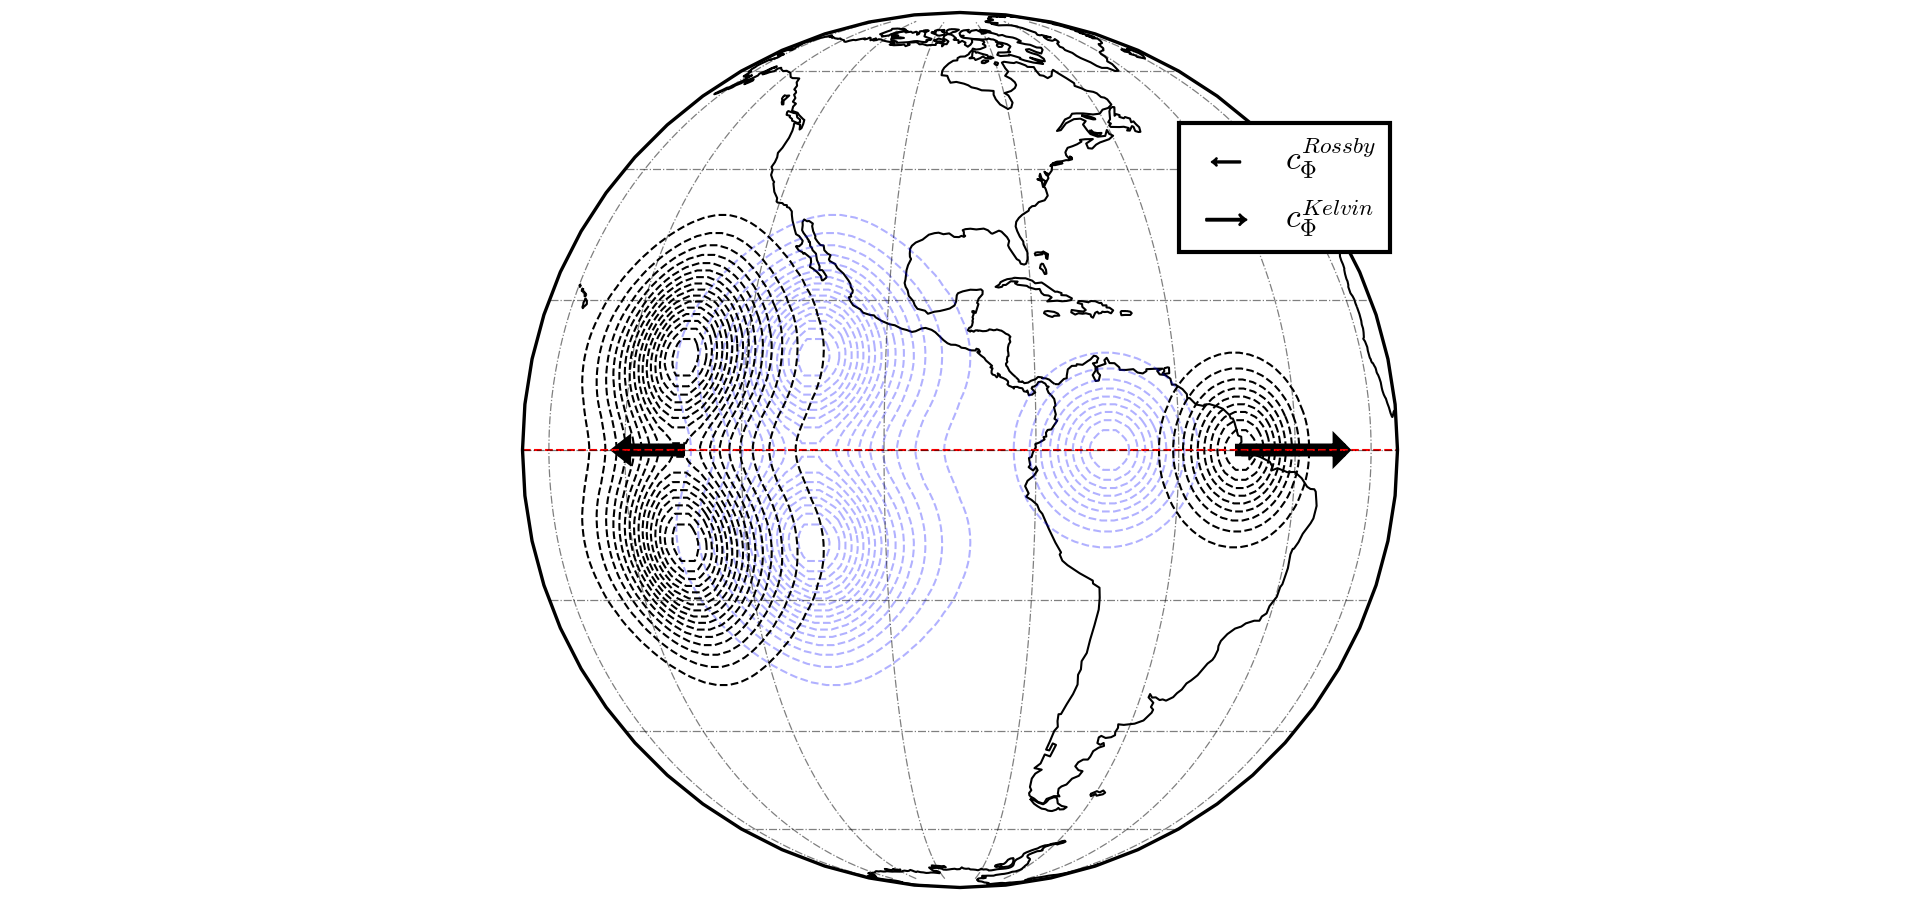
\includegraphics[width=2\linewidth]{./figure/earth_view.png}
        \caption{\footnotesize{Earth view of the equatorial domain, with the different waves propagating, the left one is a Rossby soliton and the right one is a Kelvin , note that the phase speed of the Kelvin wave is much higher than the one of the Rossby wave.}}
        \label{fig:}
    \end{figure}

    \subsection{Beta plane approximation}
    The \textbf{Beta plane approximation} consists of linearizing the Coriolis term in the shallow water equations. This approximation is valid for small latitudes, in the case of large latitudes this approximation can be replaced by the $f$ plane approximation, discussed bellow.
    The Beta plane approximation is given by the following equation:
    \begin{equation*}
        f = \beta y
    \end{equation*}
    This allows us to simplify the shallow water equations \ref{eq:1} defining the following scales parameter and the \textbf{Lamb parameter} $$E = \frac{\beta^2a^4}{ga_0}$$ Where $a$ is the radius of the earth and $a_0$ the homogenous fluid depth.

    \begin{center}
        \begin{tabular}{ccccc}
            \toprule
            \multicolumn{5}{c}{Characteristic scales}                                                                                        \\
            \cmidrule{1 -5}
            $L$                 & $T$                        & $\epsilon$                      & $\tau$                 & $\xi$              \\
            \midrule
            $\frac{a}{E^{1/4}}$ & $\frac{E^{1/4}}{2 \Omega}$ & $\frac{(2\Omega a)^2}{ga_0}$ ns & $\epsilon^{1/2}(x-ct)$ & $\epsilon^{3/2}t $ \\
            \bottomrule
        \end{tabular}
    \end{center}
    Assuming that the development of the $u$, $v$ and $h$ are of the following form:
    \begin{equation*}
        \begin{cases}
            u = \epsilon(u^0 + \epsilon u^1 + \epsilon^2 u^2 + \dots)       \\
            v = \epsilon^{3/2}(v^0 + \epsilon v^1 + \epsilon^2 v^2 + \dots) \\
            h = \epsilon(h^0 + \epsilon h^1 + \epsilon^2 h^2 + \dots)
        \end{cases}
    \end{equation*}
    The factor $\epsilon^{3/2}$ expressing that north-south current are much smaller that east-west current, for long wave [cite]
    Then we can find the following equations, at first order, after rescaling the equations \ref{eq:1} and using the slow variables $\tau$ and $\xi$:

    \begin{equation}
        \label{eq:2}
        \begin{cases}
            -c \partial_\xi u^0 -  y v^0 = -\partial_\xi h^0 \\
            y u^0 + \partial_y h^0 =0                        \\
            -c \partial_\xi h^0 + \partial_\xi u^0+ \partial_y v^0 =0
        \end{cases}
    \end{equation}
    Then we got the following reduction :

    \begin{equation}
        \label{eq:3}
        \partial_{yy} v^0 + (\frac{-1}{c} - y^2)v^0 = 0
    \end{equation}
    These first order equation leads to the following solution (Lindzen, 1967) :
    \begin{equation}
        \label{eq:Rossby}
        \begin{cases}
            v^0(y, \xi, \tau) = \partial_\xi \eta(\xi, \tau) e^{-(1/2)y^2}H_n(y)                                     \\
            u^0(y, \xi, \tau) = \eta(\xi, \tau) [ \frac{H_{n+1}(y)}{2(1-c)} - \frac{nH_{n-1}(y)}{1 +c}]e^{-(1/2)y^2} \\
            h^0(y, \xi, \tau) = \eta(\xi, \tau) [ \frac{H_{n+1}(y)}{2(1-c)} + \frac{nH_{n-1}(y)}{1 +c }]e^{-(1/2)y^2}
        \end{cases}
    \end{equation}
    With $c = \frac{-1}{2n + 1}$, $H_n$ is the physicist Hermite polynomial of order $n$. $\eta(\xi,\tau)$ is determined by the analysis of the first order solution, by solving the \textbf{KDV equation} :
    \begin{equation}
        \label{eq:5}
        \partial_\tau \eta + \alpha_n \eta \partial_\xi \eta +\beta_n \partial_{\xi \xi \xi} \eta = 0
    \end{equation}
    \cite{Boyd80}, where $\alpha_n$ and $\beta_n$ are mode dependent constant.

    The global solution regardless orders of $\epsilon$ was expressed by Holton (1973) \cite{Holton}, and get rid of the spurious roots for $n=0$ leading to \textbf{mixed Rossby-gravity waves}.
    \begin{equation}
        \label{eq:6}
        \begin{cases}
            v(\xi) = V_ne^{-(1/2)y^2}H_n(\xi)                                                                                                                                  \\
            u(\xi) = i\frac{V_n \epsilon^{1/4}}{\sigma}[ \frac{H_{n+1}(\xi) /2 }{\epsilon^{1/2} - k / \sigma} - \frac{nH_{n-1}(y)}{\epsilon^{1/2}+ k / \sigma}]e^{-(1/2)\xi^2} \\
            h(\xi) =-i\frac{V_n \epsilon^{-1/4}}{\sigma}[ \frac{H_{n+1}(y) / 2}{\epsilon^{1/2} - k / \sigma} + \frac{nH_{n-1}(y)}{\epsilon^{1/2} +k / \sigma}]e^{-(1/2)\xi^2}
        \end{cases}
    \end{equation}
    \begin{figure}[H]
        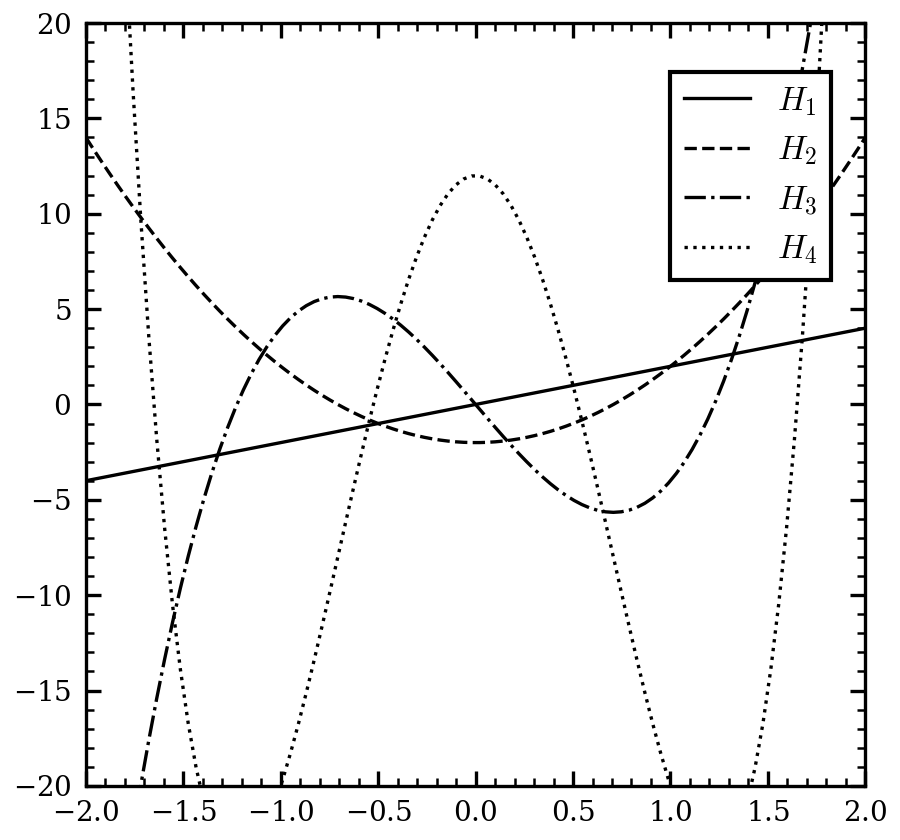
\includegraphics[width=\linewidth]{./figure/hermite.png}
        \caption{\footnotesize{The first 5 Hermite polynomials in addition to so being an orthogonal set of polynomials and a basis of $\mathcal{L}^2(\mathbb{R})$, are satisfying the following differential equation, useful to solve the equation \ref{eq:3}. }}
        \label{fig:}
    \end{figure}
    $$\partial_{yy} H_n + (\frac{-1}{c} - y^2)e^{-(1/2) y^2)}H_n(y) = 0$$ with $c = \frac{-1}{2n + 1}$
    Here k stands for the zonal wave number (\emph{wave vector along latitude}), and $\sigma$ the non-dimensional frequency using $T$. The equivalent dispersion equation of $c = \frac{-1}{2n + 1}$ is then given by:
    \begin{equation}
        \label{eq:7}
        \sigma^3 = \sigma [k^2 \epsilon^{-1} + \epsilon^{-1/2}(2n + 1)] + k\epsilon^{-1}
    \end{equation}s
    As the dispersion relation is cubic in $\sigma$, we can expect three roots for each mode $n$, hence, we must have three branches of dispersion relation, leading to different types of waves, weather dispersive or not.
    Furthermore, in the limit $n \mapsto 0$ the spurious roots of the previous dispersion relation are in the equivalent parametric equation the following:
    \begin{equation*}
        \sigma = \frac{\epsilon^{-1/2}}{2} \pm \left[\frac{ k^2\epsilon^{-1} }{ 4 } + \epsilon^{-1/2} \right]^{\frac{ 1 }{ 2 } }
    \end{equation*}
    These spurious roots give rise to the mixed Rossby-gravity waves, the positive roots stands for a high-frequency eastward moving inertia
    gravity wave, and the negative one for a strongly dispersive Rossby wave propagating westward.
    \begin{figure}[H]
        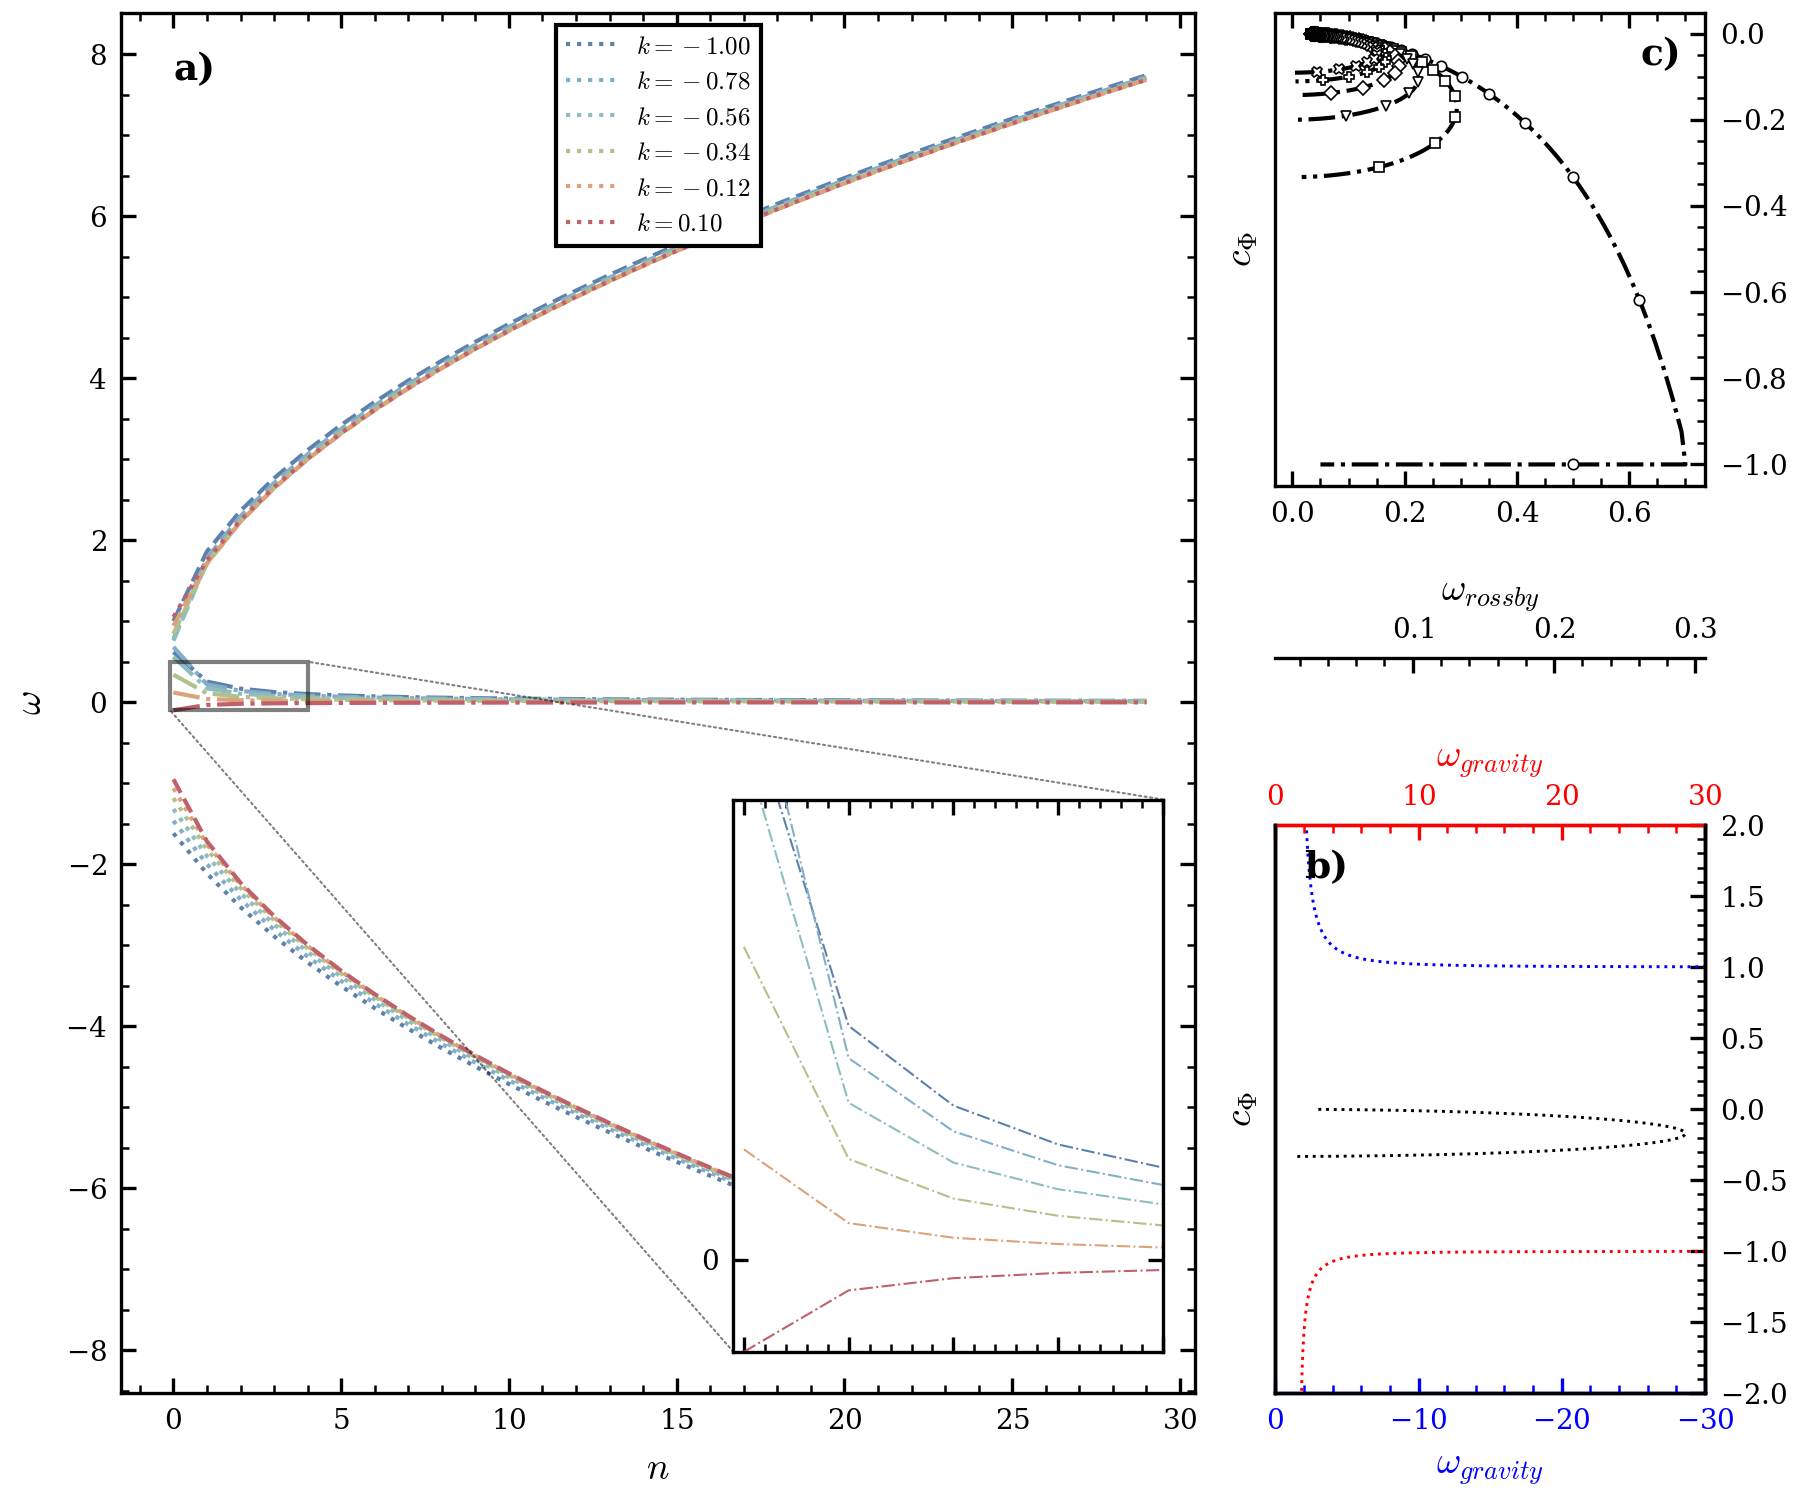
\includegraphics[width=\linewidth]{./figure/roots.png}
        \caption{\footnotesize{The frequency roots of the dispersion equation are given by the fig : 1.4.a), the roots are given for a wide range of modes [0,20], and five zonal wave numbers. The three branches that appeared for relatively high modes are diverging near the mode 0, which is due to the fact that low mode are
                \textbf{weakly dispersive}, thus the phase speed is almost constant propagating westward as indicates the negative phase speed. This clarifies our domain of study, to observe weakly dispersive waves, we will study the behavior of the waves for $n$ small. The fig : 1.4.b) shows the roots for $n = 1$, the three behaviors of the roots are clearly visible and stand for gravity wave for the red and blue curve and Rossby wave for the black curve, gravity waves are non-dispersive with a phase speed $c_\Phi^{gravity} = \sqrt{ga_0}$ in the limits of relatively small frequency and Rossby waves are low frequency and  weakly dispersive. The fig 1.4.c)
                shows that Rossby waves phase speed is decreasing with the mode number, hence to study this type of waves we will focus on the mode $n=1$ the mode $n=0$, is a Rossby-gravity wave mixed and is not of particular interest to us.
                Indeed, the mode $n=0$ appears to be \textbf{strongly dispersive and dissipative}, which should imply more difficulties  for setting a reliable numerical scheme.}}
        \label{fig:}
    \end{figure}
    \subsection{Gravity waves}
    Gravity waves are solutions of the basic set of shallow water equation where the \textbf{dependency over the Coriolis term is neglected}.
    This leads to the following set :
    \begin{equation}
        \label{eq:8}
        \begin{cases}
            \partial_t u  = -g \partial_x h \\
            \partial_t v = -g \partial_y h  \\
            \partial_t h + a_0( \partial_x u + \partial_y v) = 0
        \end{cases}
    \end{equation}
    which can be reduced to the simple wave equation with $a_0$ constant :
    \begin{equation}
        \label{eq:9}
        \Box h = 0
    \end{equation}
    This type of wave are valid solution of to the equation \ref{eq:1} for high value of zonal number, i.e. for relatively small spatial scale, in order to be able of neglecting the Coriolis term.
    \begin{figure}[H]
        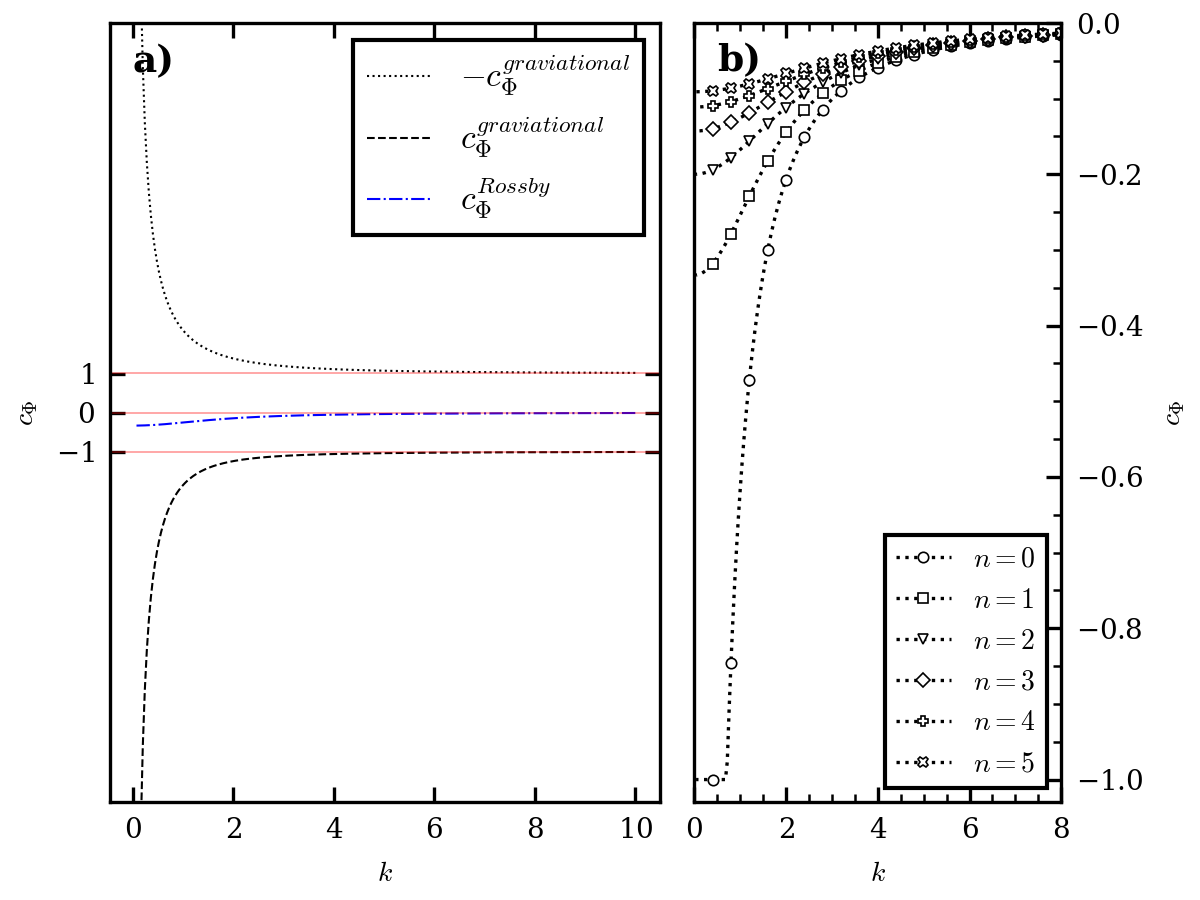
\includegraphics[width=\linewidth]{./figure/roots_k.png}
        \caption{\footnotesize{The fig 1.5.a) shows the dependency of the phase speed over the zonal wave number. Here the three branches correspond to the same wave type as before, this highlights the need to have large scale wave with low zonal wave number to have weakly dispersive Rossby waves. The fig 1.5.b is quite redundant with the fig 1.4.c)
                showing that independently of the zonal wave number the mode number plays a great role in Rossby waves phase speed. However, the propagation is \textbf{always westward}, regardless of parameters.}}
        \label{fig:}
    \end{figure}
    \subsection{Rossby waves}
    As the two previous figures highlight it, the Rossby waves are weakly dispersive and propagate westward along the equator, their phase speed is decreasing over their zonal wave-number, and the mode number. Hence, the first mode we will be studied here,
    the $\eta$ function is then given by the following equation :
    \begin{equation}
        \label{eq:8}
        \eta(\xi, \tau) = A \text{sech}^2[B(\xi - 0.395B^2\tau)]
    \end{equation}
    with $A = 0.772 B^2$, to be in the same scope as Boys we will take $A = 0.12$ for height amplitude, so it gives us $B = 0.394$. Let's recall that $$c_\Phi = \frac{-1}{2n + 1} = -\frac{1}{3}$$ in our case. Here B stands for a zonal number like. It's clear that with these parameters ranges we are definitely in the strong Rossby wave domain as $k<1$ and $n<10$.
    \begin{figure}[H]
        \hspace*{-.5cm}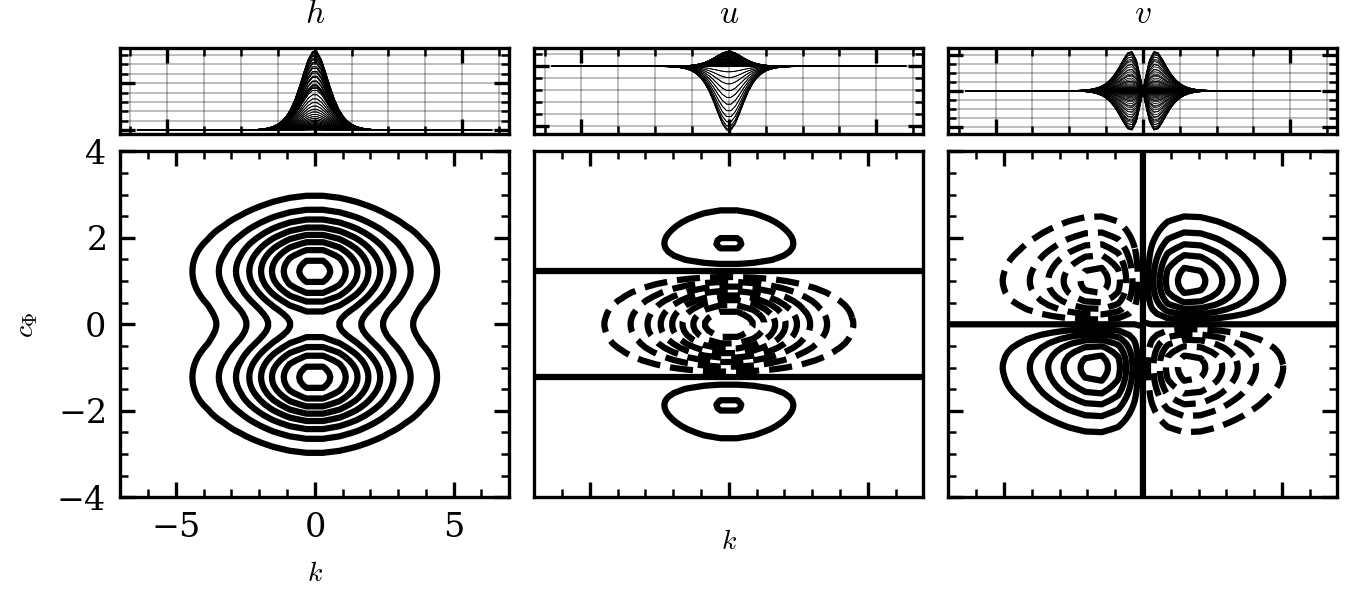
\includegraphics[width=1.1\linewidth]{./figure/initial_data.png}
    \end{figure}
    \captionof{figure}{Initial Rossby wave soliton $n=0$ $u$, $v$ and $h$ fields, for the parameter of $\eta(\xi, \tau)$ described above. As we can see through the initial condition the wave should propagate westward through a Coriolis pumping effect describe in the following figure. The westward movement is induced by the initial westward motion of the u-field,
        which is maintained by a \textbf{Coriolis cycle} in the v-field.}

    \begin{figure}[H]
        \centering
        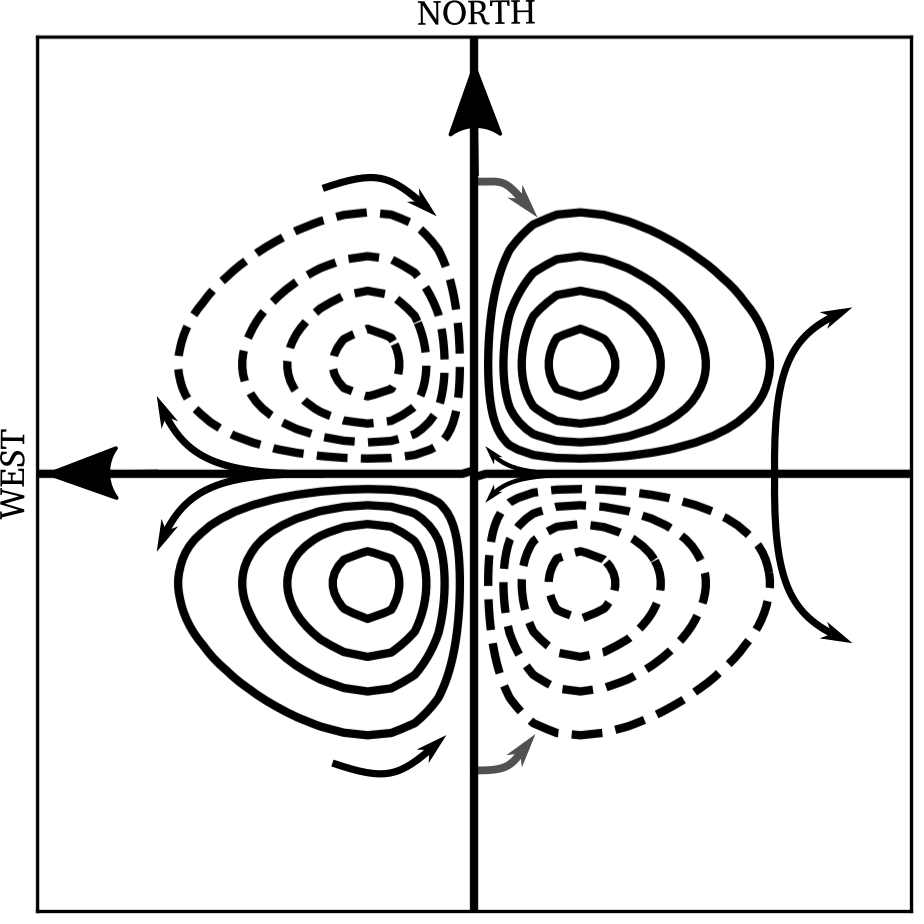
\includegraphics[width=.8\linewidth]{./figure/pump.png}
        \vspace*{.5cm}
        \caption{\footnotesize{This figure lays the emphasis on the v-field pumping effect : westward nodes are driving the flow westward and at the first order the eastward flow should be driven eastward. However, through a second order perturbation study, we can see that the eastward flow is driven southward and westward flow northward at the Northern-hemisphere,
                which introduce a pumping effect with a periodic inversion of the v field driving nodes, in gray the eastward flow driving the pumping effect. However,  as Boyd underlined it, this non-linearity are creating soliton but not solitary waves, indeed here, the soliton should develop a \textbf{wave train tail}. The second order Coriolis effect is driving east nodes to north in the northern-hemisphere and to south in the southern-hemisphere.}}
        \label{fig:vfield Rossby}

    \end{figure}

    \subsection{Kelvin waves}
    Kelvin equatorial wave are a particular solution type of the beta-plane model discovered by Wallace and Kousky (1968a), they are propagsting eastward and are non dispersive such as gravity waves, with a phase speed $$c_\Phi^{Kelvin} = \sqrt{ga_0}.$$ This behavior results from considering a \textbf{zero vertical velocity component} $v(\xi) = 0$ in the equations \ref{eq:6}, which leads to the following equation :
    $$\xi u =- \epsilon^{\frac{1}{2}}\partial_\xi h$$
    which gives solution to the following solutions\cite{Holton} :

    \begin{equation}
        \label{eq:9}
        \begin{cases}
            u(\xi) = U_{-1}e^{-(1/2)\xi^2} \\
            v(\xi) = 0                     \\
            h(\xi) = U{-1}\frac{\sigma}{s}e^{-(1/2)\xi^2}
        \end{cases}
    \end{equation}
    This is equivalent of the equation set \ref{eq:6} with $n=-1$ and $V_{-1} = -2i\epsilon^{-\frac{1}{4}}s U_{-1}$.
    \begin{figure}[H]
        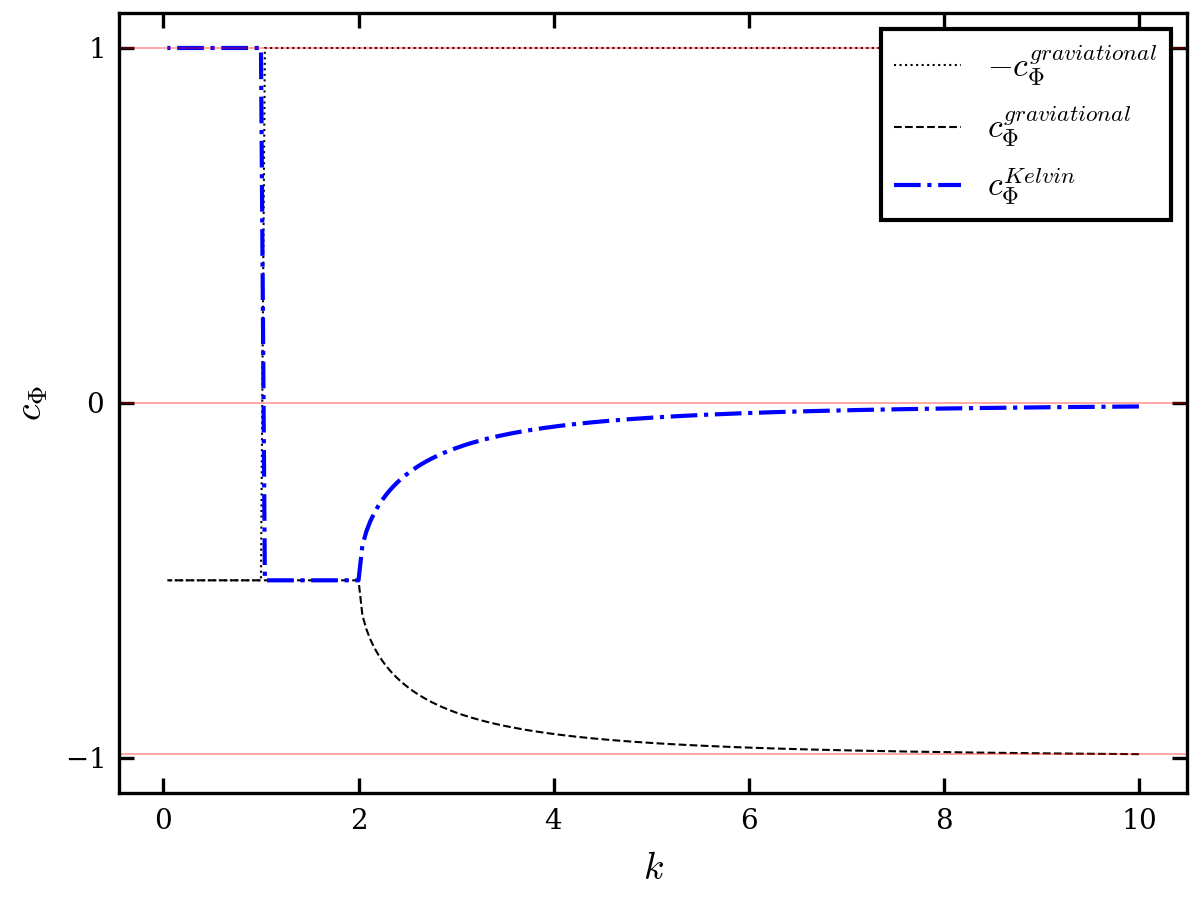
\includegraphics[width=\linewidth]{./figure/roots_k2.png}
        \caption{\footnotesize{The dependency of the phase speed for the mode $n = -1$ over the nodal wave number shows that the roots corresponding to kelvin wave exists only for $k<1$, i.e. for large spatial scale, we find the same conclusion as before
                for localized spatial scale the soliton are gravitational wave propagating westward, or eastward, for intermediate values we observe a mixed kelvin-gravity wave.}}
        \label{fig: Kelvin mode}
    \end{figure}
    \chapter{Numerical methods}
    These specific set of Poincarré waves solution present no \textbf{damping effect}, hence they are a good way to evaluate the efficiency
    of a numerical integration scheme, indeed the only source damping effect will be due to numerical errors. This numerical error can be evaluated by comparison of the real solution that can be difficult to obtain, and the numerical solution.
    This is why it will be relevant to use conservation of mass and energy to evaluate the model, and to evaluate the damping effect of the scheme.
    \section{Integration scheme}
    Our scheme will be based on simple \textbf{Chebyshev spectral method} on a non normalized domain, i.e. $[-1,1]$. This choice is motivated by the fact that spectral method are quite precise and fast for computing gradients, which is an important part of the shallow water equations.
    Furthermore, the non normalized domain is necessary to be in the range of the Rossby wave soliton in the scope of Boyd study. Indeed, from 1.10 we got the following nodal number $B = .394$, implies that the wave width will be $\sim 1$ this is why we have to take a larger mesh.
    \subsection{Spatial discretization}
    The spatial discretization is done with the Chebyshev-Gauss collocation points on $[-1,1]^2$. Then we multiply each component of the CGL nodes to be in the desired range of study, by the linear change.
    $$x'_{i,j} = (\alpha \cos(\frac{i\pi}{N}), \beta \cos(\frac{j\pi}{N}))$$
    To be in the following range : $[-\alpha, \alpha] \times [-\beta, \beta]$. Here we will choose $\alpha = 24, \, \beta = 4$
    This gives the following mesh :
    \begin{figure}[H]
        \hspace*{-.5cm}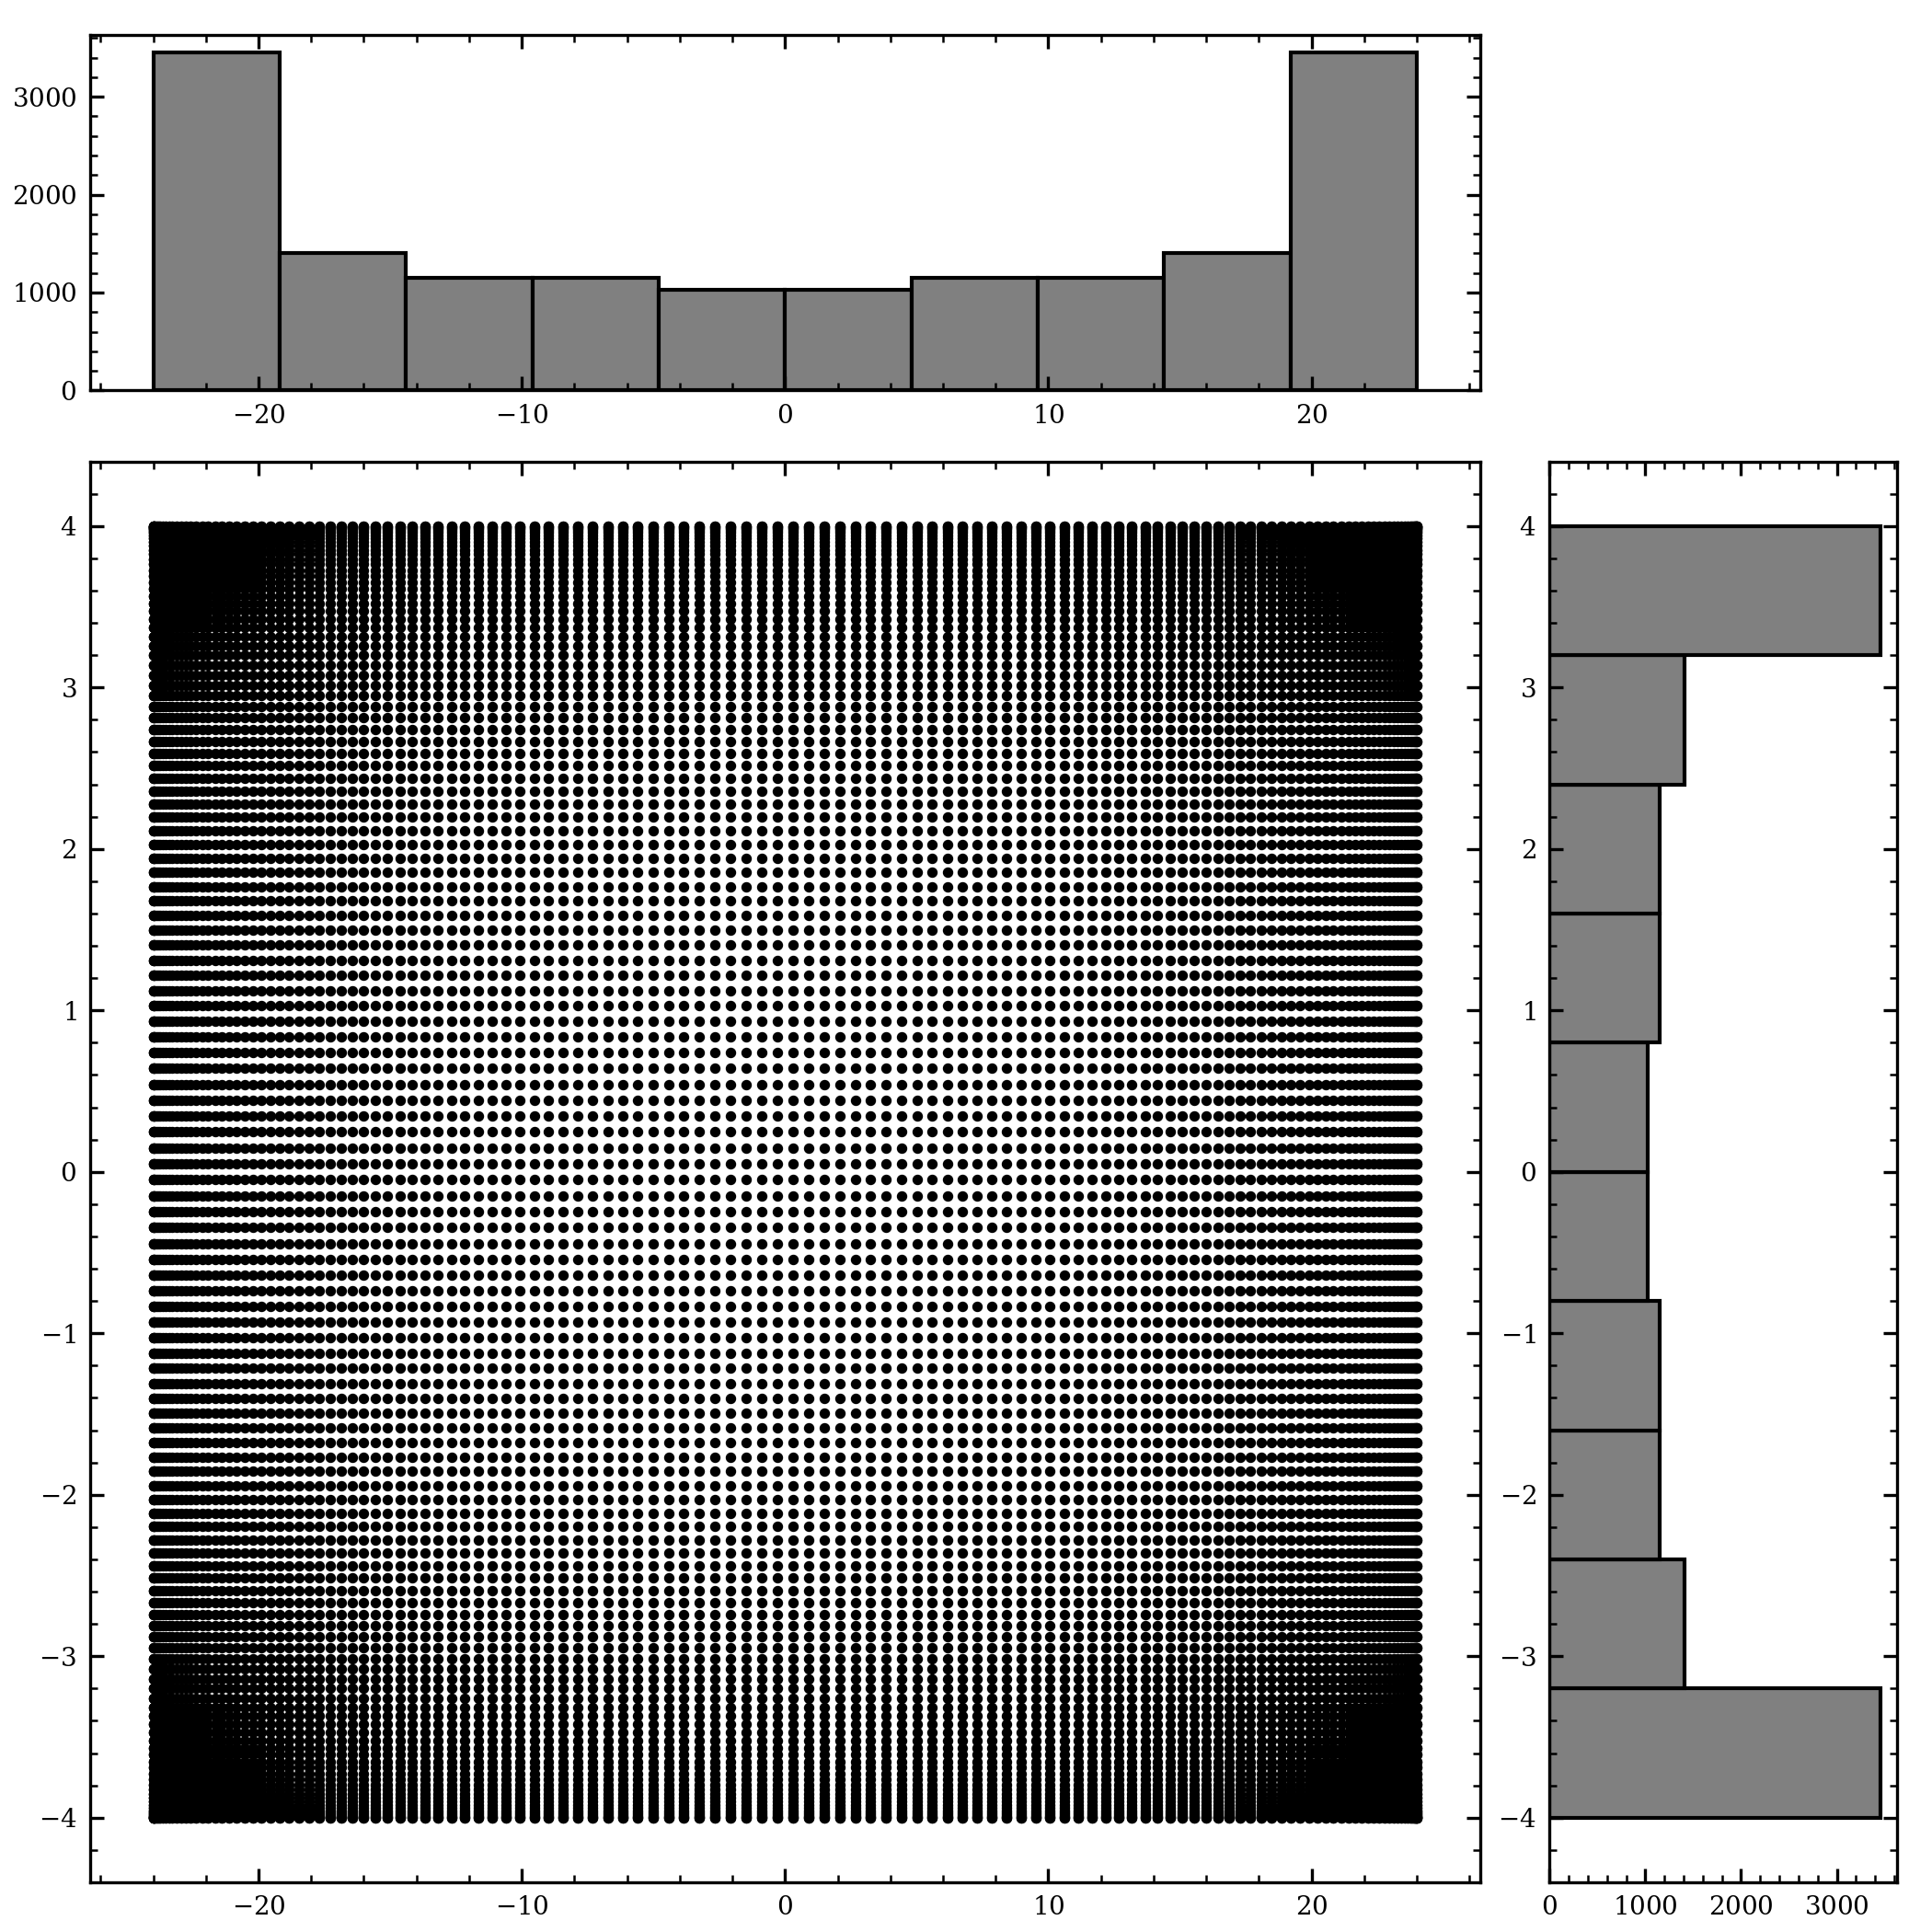
\includegraphics[width=1.1\linewidth]{./figure/mesh.png}
        \caption{From this figure we can suggest the strong mesh refinement on the edge (due to the spectral method) will imply strong conditions on the time discretization due to the CFL condition ($\Delta t \le C N^{-2}$) imposed by the wave propagation. We will study the
            CFL condition in the next part}
        \label{fig: mesh}
    \end{figure}

    \subsection{Time discretization}
    The time discretization is done with a simple \textbf{leap-frog like} method. This consists of the 2 steps size scheme for time derivative :
    $$\partial_t u(t) \approx \frac{u(t + \Delta t) - u(t - \Delta t)}{2\Delta t}$$
    This scheme is second order accurate in time, indeed let's consider the following expansion :

    $$u^{(n+1)}_{\text{LF}}=u^{(n-1)}_{\text{LF}}+2h\,\left(f(nh,u^{(n)}_{\text{LF}})\right),$$
    Denoting by $\tilde u^{(n+1)}$ the value of the right-hand side obtained by inserting a smooth solution $u$ of the ordinary differential equation  into the above scheme, one gets, using a Taylor expansion :
    \begin{multline*}
        \tilde u^{(n+1)}=u(t_n)+h\,f(t_n,u(t_n))\\
        +\frac{h^2}{2}\left(\frac{\partial f}{\partial t}(t_n,u(t_n))+f(t_n,u(t_n))\frac{\partial f}{\partial x}(t_n,u(t_n))\right) \\
        +O(h^3)
    \end{multline*}
    This matches the Taylor extension up to order 2 of the hypothetical solution $u$. Hence, the local truncation error : $\delta^h_n \underset{h \rightarrow 0}{=} O(h^3)$. The method is then second order accurate in time.
    This discretization results in the following scheme :
    \begin{equation}
        \label{eq:10}
        \begin{cases}
            u^{n+1}  = u^{n-1} + 2\Delta t -g \partial_x h^n + fv^n \\
            v^{n+1}  = v^{n-1} + 2\Delta t -g \partial_y h^n - fu^n \\
            h^{n+1}  = h^{n-1} - 2\Delta t a_0( \partial_x u^n + \partial_y v^n) = 0
        \end{cases}
    \end{equation}
    \subsection{CFL condition}
    To set the convergence condition of Courant–Friedrichs–Lewy (CFL), we have studied the behavior of the simulation through multiple discretization in time and in space,
    And as exposed before the \textbf{CFL conditions} is strongly impacted by the spectral mesh with irregular spacing Fig\ref{fig: mesh}. Indeed, as the mesh refinement is strong on the edge, the time discretization must be as well, (this duration must be less than the time for the wave to travel to adjacent grid points).
    Generally the CFL condition is given by the following equation :
    $$C=\Delta t\left(\sum _{i=1}^{n}{\frac {u_{i}}{\Delta x_{i}}}\right)\leq C_{\max}.$$
    With $u_i$ the i-th amplitude component of the speed. Here we will study the westward propagating Rossby wave soliton, hence the $u_1$ is the only non-zero component of the velocity.
    So we got the following CFL condition :
    $$C=\Delta t\left(\frac {u_{1}}{\Delta x_{1}}\right)\leq C_{\max }.$$
    Here $\Delta x_1$ is the distance between two adjacent grid points, as it is not uniform we will take the minimum distance, which is the one on the edge of the domain, yet on the edge we have the following :
    $$\Delta_x = 1 - \cos(\frac{1}{N}) \approx \frac{1}{N^2}.$$
    Furthermore, as we will study the behavior of the mode $n=1$, with a theoretical phase speed $c_\Phi = u_1 = -\frac{1}{3}$. Then we got :
    the following condition : $\Delta_t \le 3C_{\max} N^{-2}$
    \begin{figure}[H]
        \centering
        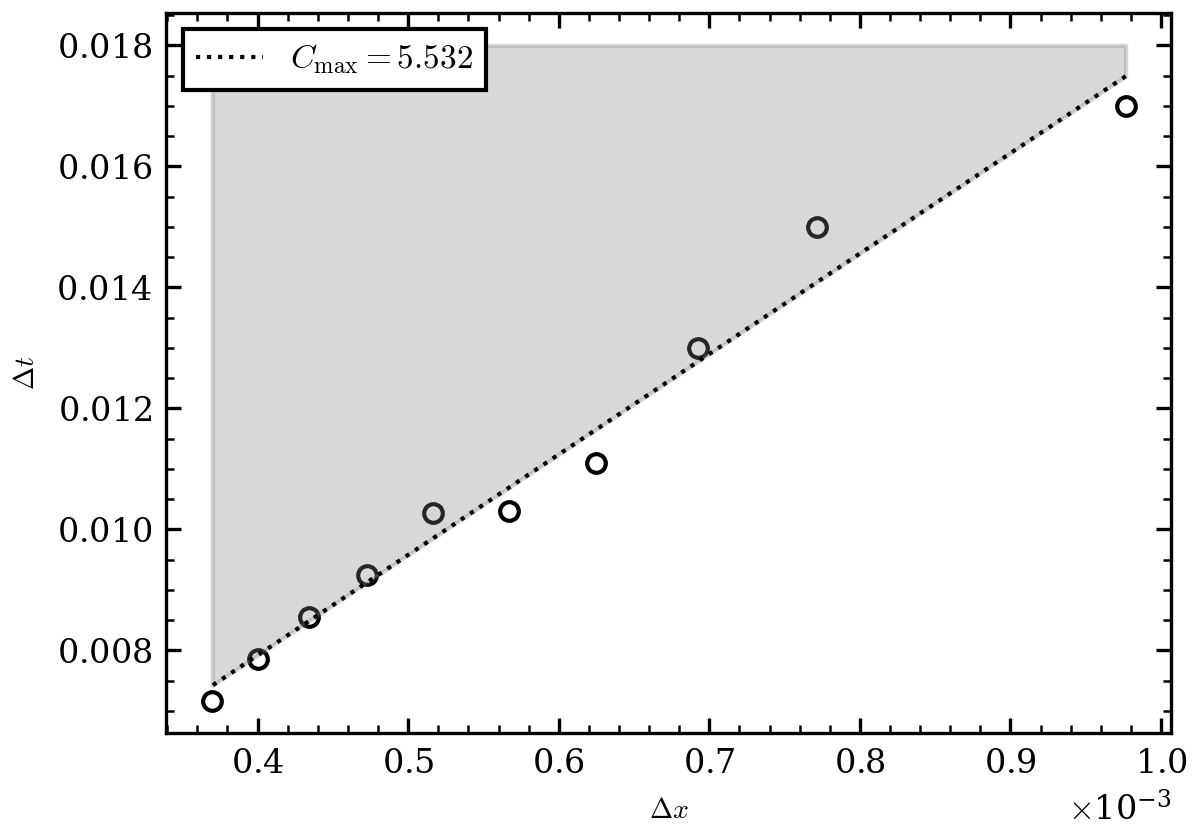
\includegraphics[width=1\linewidth]{./figure/dt_dx.png}
        \caption{Here we determined $C_{\max} = 5.532$ using many, time and space discretization, the divergence criterion was the follwing, if the soliton height is higher than its original height $h_0 = 1.12$, then the simulation is said to be non-convergent,
            The plotted value are the limits value of convergence obtained for discretized $\Delta x, \Delta t$.}
        \label{fig:CFL}
    \end{figure}
    \subsection{Boundary Condition}
    Hence, we used a Chebyshev spectral methods we cannot use periodic boundary condition. One goal of this study is to evaluate the phase speed of the Rossby wave soliton, hence we must choose a wide box to avoid boundary effects especially over the horizontal direction, to study the behavior of the wave on a wide time domain.
    For the simulation the \textbf{Simple Dirichlet boundary condition} is used, i.e. $h = v = u = 0$ on the boundary. This is satisfying the kinematic conditions and the dynamic ones :
    water particles will not cross either boundary for the kinematic condition, and the dynamic condition is a no slip one.
    \subsection{Conservation of mass and energy}
    The conservation of mass and energy are important to evaluate the efficiency of the numerical scheme, indeed let's recall that the only damping effect is due to the numerical error, hence the conservation of mass and energy will be a good indicator of the efficiency of the scheme.
    The mass conservation tackled the kinematic condition, as no water particle should cross the boundary, and the energy conservation is a good indicator of the numerical error.

    \subsubsection{Conservation of mass}
    The total mass is given by the following discretized equation :
    $$M = \sum_{i,j} (a_0 + h_{i,j})\Delta x_i \Delta y_j$$
    This equation supposed a homogenous and incompressible flow which is easily verified in the shallow water field.

    \subsubsection{Conservation of energy}
    The total energy is given by the following discretized equation~:
    $$\tfrac{1}{2}\sum_{i,j}(u_{ij}^2 + v_{ij}^2 + ((a_0 + h_{ij}))g) (a_0 + h_{ij}) \Delta x_i \Delta y_j$$
    This corresponds to a simple kinetic energy plus a potential energy under the same hypothesis as before.
    \subsection{Potential Vorticity}
    The potential Vorticity can be defined as the following :

    $$q = \frac{f + (\partial_x v - \partial_y u)}{h}$$
    This quantity is conserved along a stream-line in case of non dissipation and external forces, them one can define the potential enstrophy quantity which is the conserved quantity indicating the strength of the potential Vorticity.
    $$\Omega = h \frac{q^2}{2}$$
    The discretized equation is given by the following :

    $$\Omega = \tfrac{1}{2}\sum_{i,j}h_{ij}q_{ij}^2\Delta x_i\Delta y_j  $$
    The gradients will be computed using the Chebyshev spectral method.

    \section{Numerical results}
    The following simulations tackled the following cases, the first one is the propagation of a Rossby wave already studied by \cite{CF}, that will be used as a reference for the numerical scheme. The second one is the propagation of a Kelvin wave, and the third one tackled the behavior of an unstablw wave.
    In this last part we will delve into the \textbf{mode separation} of this wave and the energetic aspect of this splitting.
    \subsection{Rossby soliton waves}
    For simulating the behavior of the ref wave we used the following parameters :

    \begin{center}
        \begin{tabular}{ccccc}
            \toprule
            \multicolumn{5}{c}{Characteristic scales}    \\
            \cmidrule{1 -5}
            $a_0$ & $\beta$ & $g$    & $N$  & $\Delta t$ \\
            \midrule
            $1$   & $1$     & $1$ ns & $64$ & $2e^{-3}$  \\
            \bottomrule
        \end{tabular}
    \end{center}
    Compared to the other study the CFL conditions are quite restrictive due to the spectral methods : \cite{CF}.
    However,  we achieved to get a good convergence despite the relatively low discretization in space.
\end{multicols}
\begin{figure}[H]
    \centering
    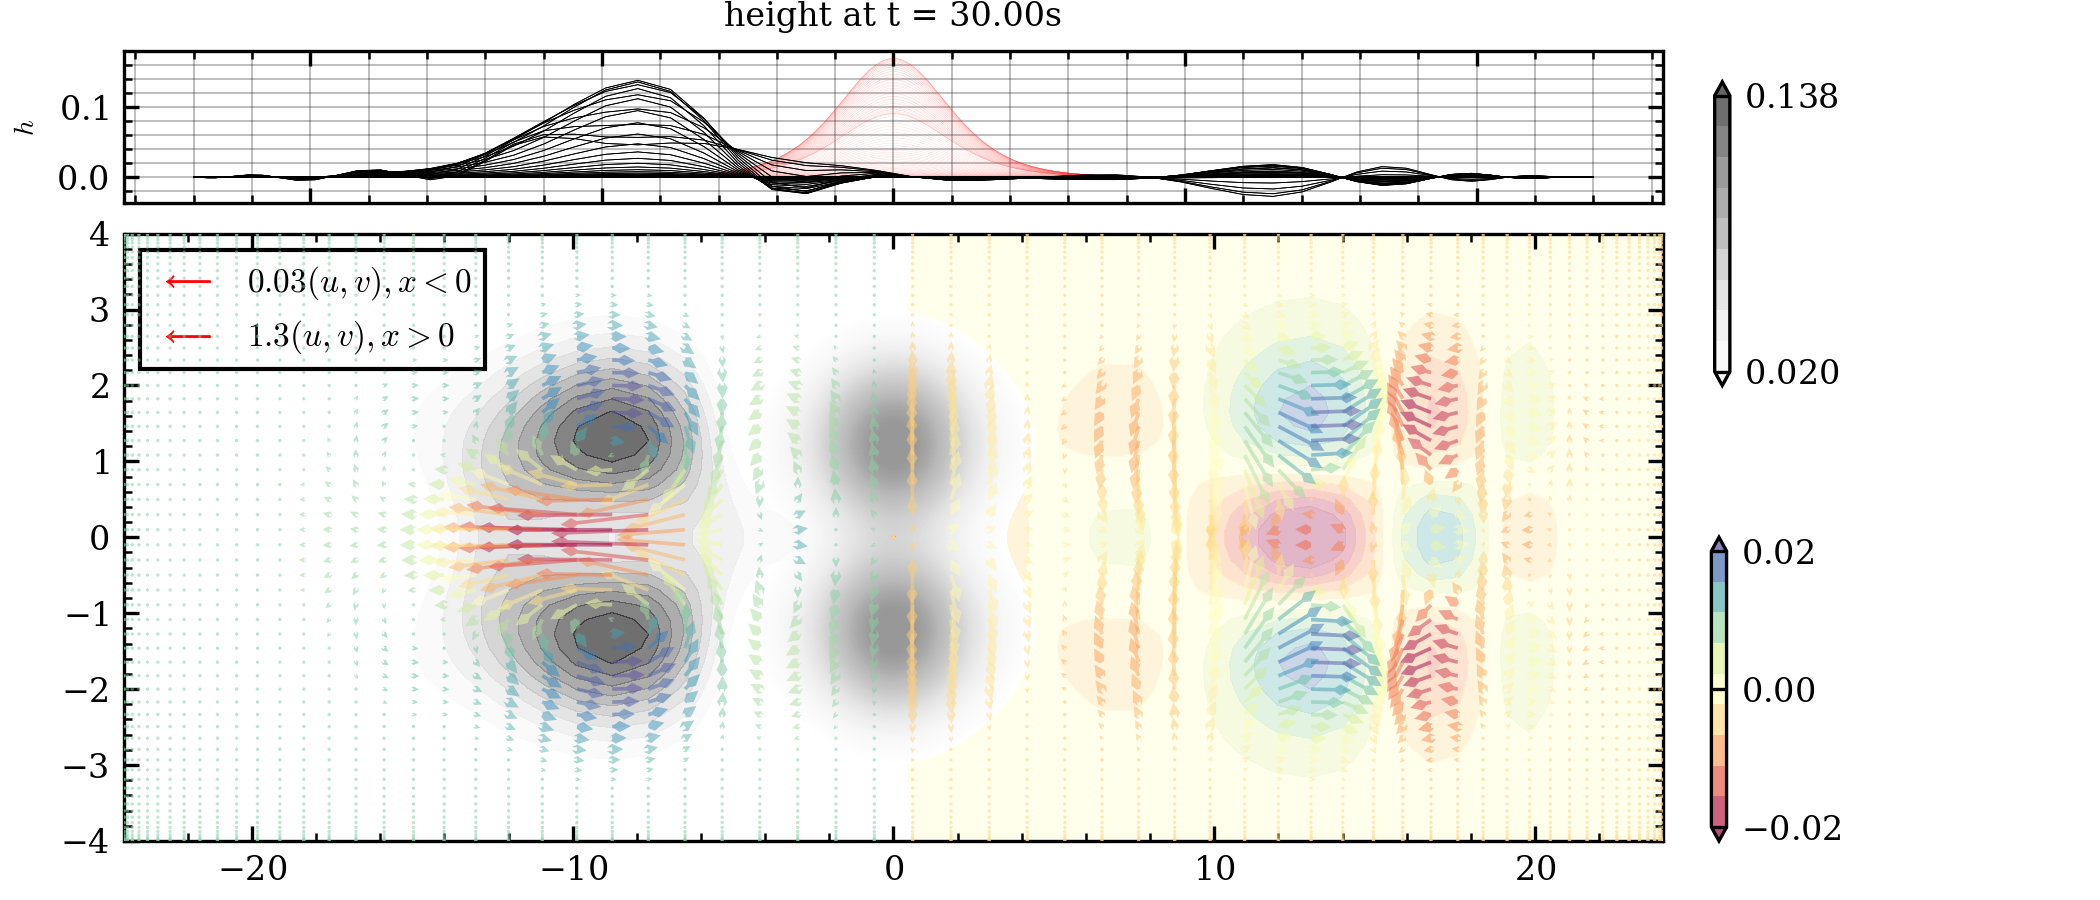
\includegraphics[width=\textwidth]{./figure/soliton.png}
\end{figure}
\captionof{figure}{The westward propagation of the soliton is clearly visible through the comparaison with the initial condition in light red. Furthermore we can see the pumping effect operate  in the velocity field, with a \textbf{strong westward flow}, The amplitude of the soliton have a slight damping effect, which is due to numerical error, and eastward propoagation of the wave train [ref]. In addition to that,
    let's denote that the eastward wave train is propagating much faster than the westward soliton, let's add that there are strongly dispersive, and should refer to Rossby-gravity wave of mode $n=0$, since they are the only Rossby-like wave propagating eastward.
    This wave train is due to non-linearity and constitutes the 2nd order response of the solitary wave to the Coriolis effect. It seems that the wave train are made from a \textbf{succession of soliton-like shape}. Indeed, they present some
    strong similarities in shape with the soliton, but with a much smaller amplitude and their propagation speed is faster, and characterized by a high dispersion. We can also highlight the sign swap for each wave train, due to the Coriolis pumping effect, hence it inverts the sign if the v-field node periodically, this can be explored through Boyd \cite{Boyd80} work. These instabilities radiations are exponential function of the Rossby soliton amplitude, this leads to an emission of radiative instabilities with amplitudes order of the $n - 2$ modes for $n \ge 3$. For $n = 1$ Williams showed that the instabilities results in radiative decays into the barotropic
    modes. Let's also note that the instabilities are not nodated directly from the soliton, but far from it, this strange behavior is also observed in other weakly non-local solitary $\Phi 4 breather$}
\begin{center}
    We have found the following equation for $n=0$ :
    \begin{equation}
        \label{eq:4}
        \begin{cases}
            v^0(y, \xi, \tau) = \partial_\xi \eta(\xi, \tau) e^{-(1/2)y^2}H_n(y)                  \\
            u^0(y, \xi, \tau) = \eta(\xi, \tau) \pm[ 0.03646482 H_0 - 0.27467347H_2]e^{-(1/2)y^2} \\
            h^0(y, \xi, \tau) = \eta(\xi, \tau)\pm[ -0.20872123 H_10 + 0.2103431H_2]e^{-(1/2)y^2}
        \end{cases}
    \end{equation}
\end{center}
\begin{multicols}{2}
    \subsubsection{Conservation of mass \& energy}
    The mass and energy conservation accounts for the quality of the numerical scheme :
    \begin{figure}[H]
        \centering
        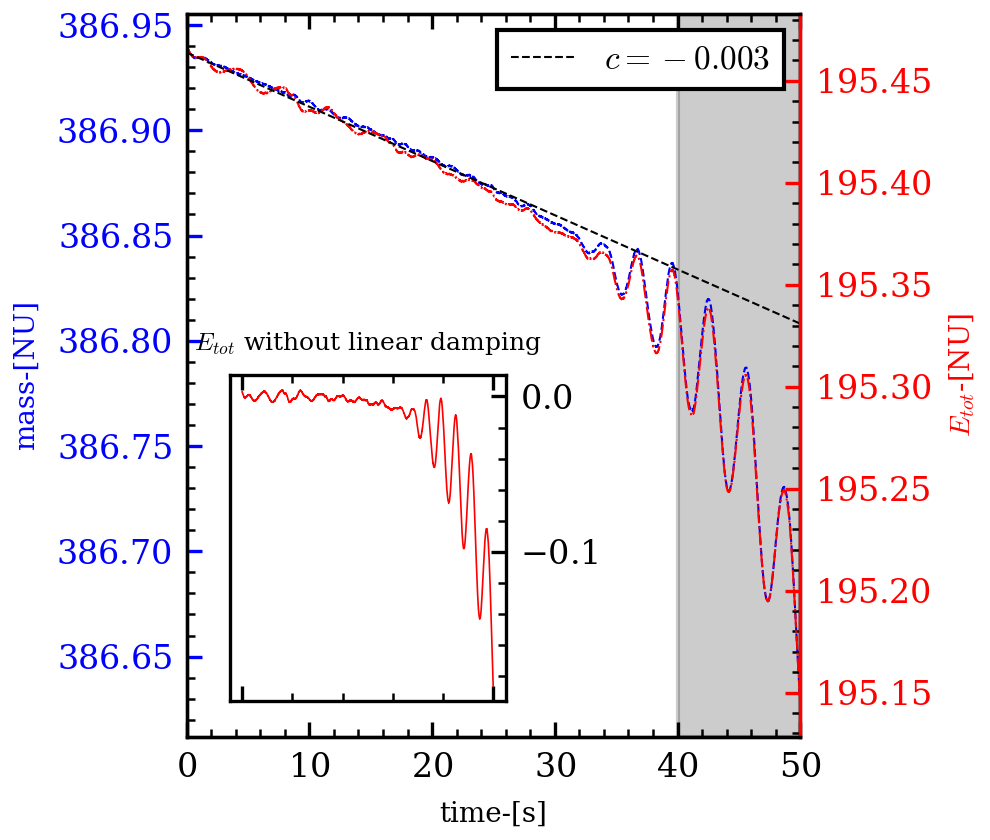
\includegraphics[width=\linewidth]{./figure/energy.png}
    \end{figure}
    \captionof{figure}{The conservation of mass and energy are quite good, the mass is conserved up to $10^{-4}$, and the energy up to $10^{-3}$, this is due to the numerical error, however let's note that the damping is quite linear during the simulation,
        and can be compared to a simple friction coefficient of value $c = 3e^{-4}$. Which unearths some question about the origin of this numerical damping.  To avoid boundary effects one can propose to introduce strong damping on the boundary, this has been studied as \emph{Sponge Layer} by Boyd \cite{Boyd2002}, and is a good way to avoid transients interferences in the main flow (Rossby soliton). Indeed, here,
        we must limit our study to $T = 40$s to avoid boundary effects, which is quite embarrassing because we must keep a fine spatial discretization to avoid numerical dispersion, and a fine time discretization to avoid numerical damping. So we cannot enlarge the spatial domain to study the wave propagation over a longer time (limit time calculation).}
    \subsubsection{Potential Vorticity}
    The enstrophy potential is a conserved quantity is our case and is extremely relevant since it allows us to dive into the potential Vorticity of the flow, since the radiative instabilities should increase, the potential Vorticity, and thus the enstrophy potential.
    Note that, even if the instabilities have small amplitudes in height they have a strong impact in the $v-field$, when the balance between linear wave dynamics and non-linearity is broken. Boyd introduced \textbf{antisymmetric parts of the wave}. Indeed, due to instabilities the vortex pair becomes asymmetric, and
    symmetrizes itself by leaving the antisymmetric part behind as a wave packet. And then the equilibrated soliton steadily translated without change in shape or amplitude, this is an important part of the dynamics for the propagation of the soliton, this is why it must be tackled.

    \begin{figure}[H]
        \centering
        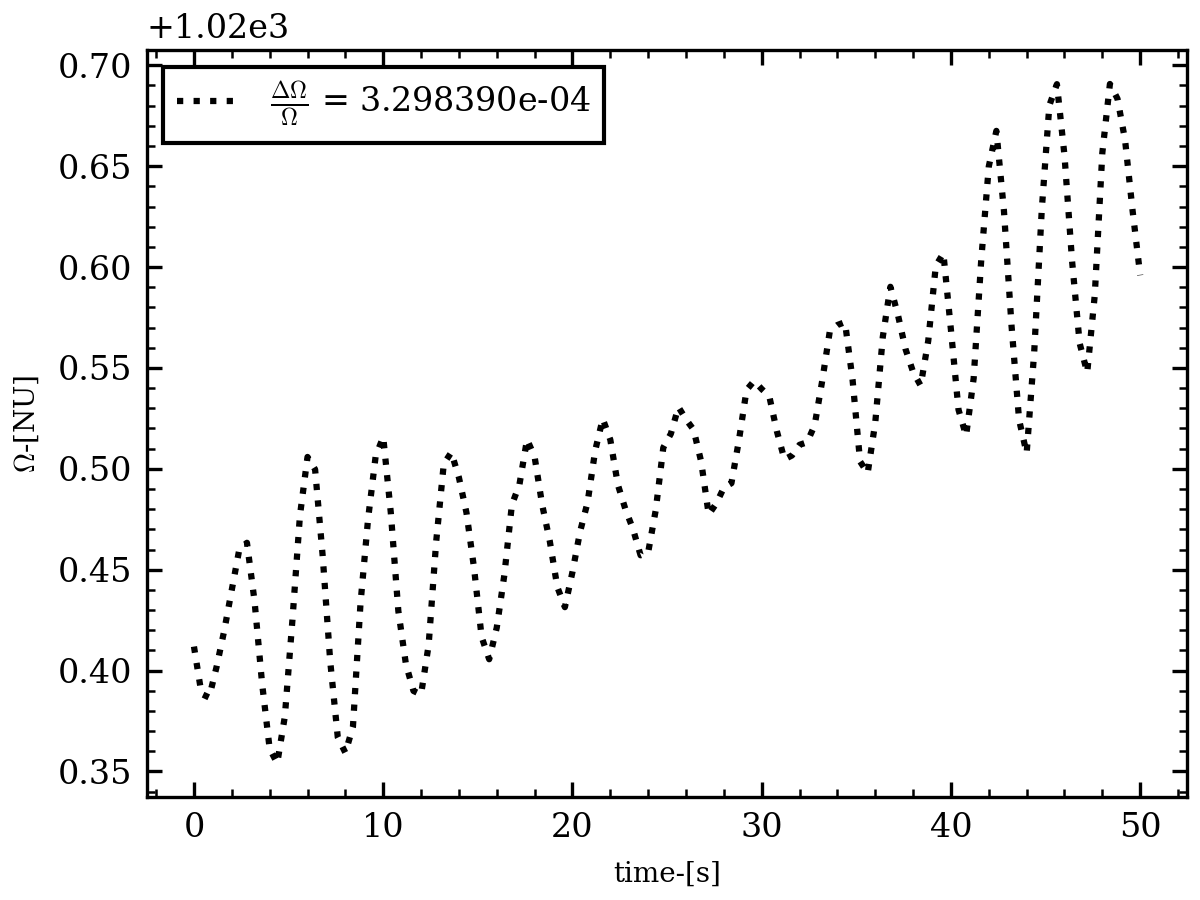
\includegraphics[width=1\linewidth]{./figure/potential_enstrophy.png}
        \caption{As intended, the enstrophy remains quite constant, with a constant increasing due to instabilities shedding, this reasonable increase is due to the negligible height of the radiations. It's reasonable to think that the oscillations in the Potential Vorticity come from
            successive nodations and dissipation of instabilities from the soliton.}
        \label{}
    \end{figure}

    \begin{figure}[H]
        \centering
        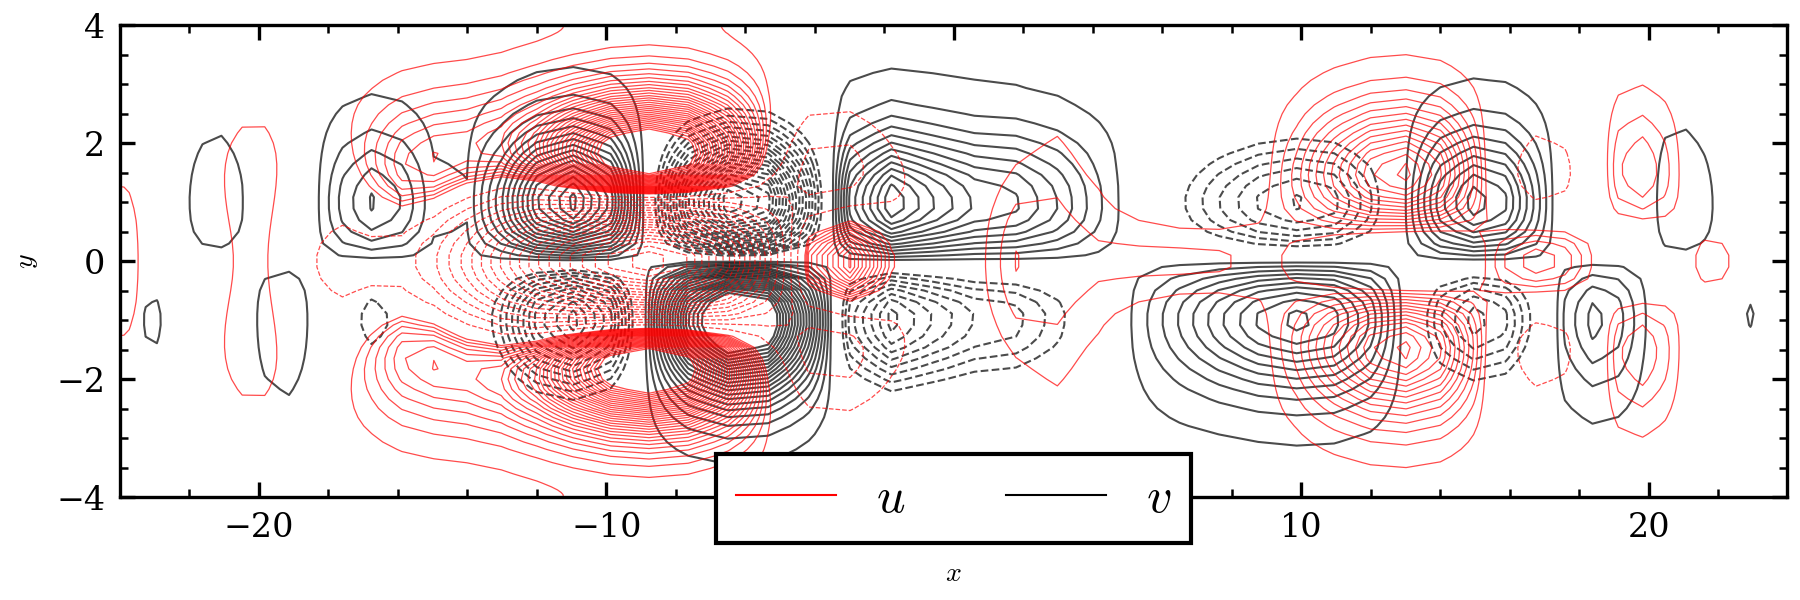
\includegraphics[width=1\linewidth]{./figure/velocity.png}
    \end{figure}
    \captionof{figure}{The radiative shedding has a great impact on the flow with strong barotropic modes (maybe $n = 0$ Rossby waves) propagating eastward with a phase speed $c_\Phi \approx 1$, in our case it matches with the Kelvin phase speed}


    \subsubsection{Phase speed evaluation}
    The phase speed is evaluated by tracking the max of the soliton shape, we introduced a moving window around it to get rid of the numerical dispersion, and then we evaluate the phase speed
    by taking the mean position of the moving window, this leads to the following :
    \begin{figure}[H]
        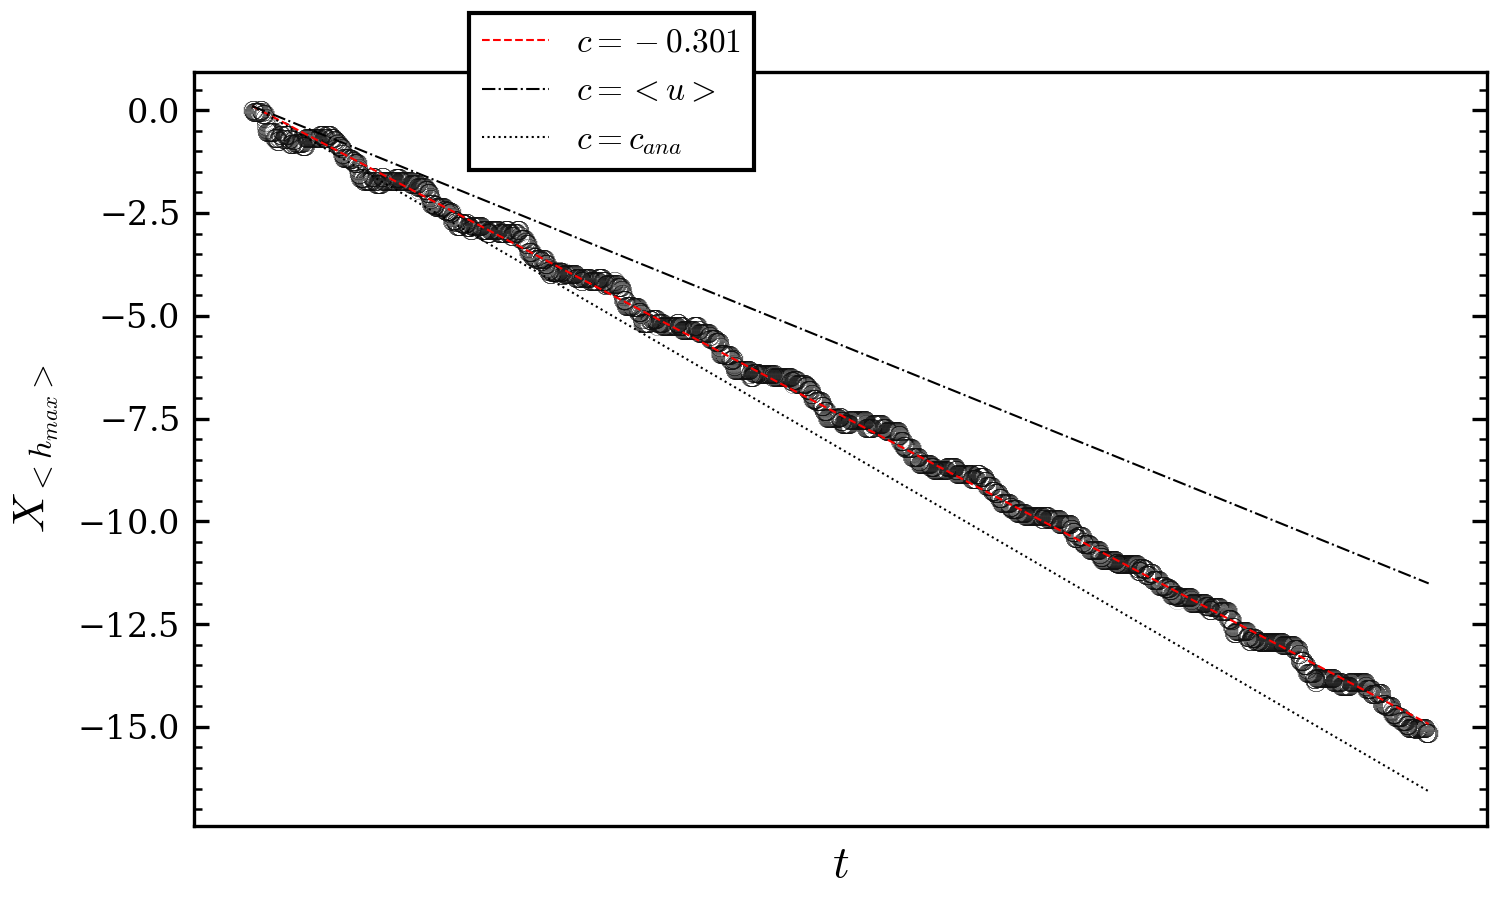
\includegraphics[width=1\linewidth]{./figure/mean_height.png}
        \caption{Phase speeds evaluation}
    \end{figure}
    The phase speed calculated, is $c_\Phi = -0.301$, which is quite close to the theoretical one $c_{ana} = -\frac{1}{3}$, this leads to the following relative speed : $$C_{num}/C_{ana} = .903$$ as defined by \cite{CF}, this is a quite good result considering the mesh refinement on the domain studied compared to the mesh size used by \cite{CF}, we will also lay the emphasis on the use of super calculator for obtaining such good result. Furthermore,  another interesting things is that,
    the phase speed is not given by the maximum of the $u$-field along the horizontal axis. Indeed, the max speed of the $u$-field is much lower than $C_{num}$. This result is quite strange, how the wave can travel faster than the velocity field allows...
    \subsection{Kelvin waves}

    For simulating the behavior a Kelvin wave we use the following parameters :

    \begin{center}
        \begin{tabular}{ccccc}
            \toprule
            \multicolumn{5}{c}{Characteristic scales}    \\
            \cmidrule{1 -5}
            $a_0$ & $\beta$ & $g$    & $N$  & $\Delta t$ \\
            \midrule
            $1$   & $1$     & $1$ ns & $64$ & $2e^{-3}$  \\
            \bottomrule
        \end{tabular}
    \end{center}

    We will take a wave of the following form, satisfying the Kelvin wave equation :
    \begin{equation}
        \label{eq:Kelvin wave}
        \begin{cases}
            h(x,y,t = 0) = H_0  \frac{\sigma}{k} \exp(- ((kx) ^2 +(ly)^ 2)) \\
            u(x.y, t = 0) = H_0 \exp(- ((kx) ^2 +(ly)^ 2))                  \\
            v(x,y,t=0) = 0
        \end{cases}
    \end{equation}
    For the simulation we will take the following parameter for the Kelvin wave defined by \refeq{eq:Kelvin wave}
    \begin{center}
        \begin{tabular}{ccc}
            \toprule
            \multicolumn{3}{c}{Parameter} \\
            \cmidrule{1 -3}
            $H_0$ & $k$   & $l$           \\
            \midrule
            $2$   & $0.5$ & $1$           \\
            \bottomrule
        \end{tabular}
    \end{center}
    Note that we took $k = 0.5$ to be in the scope of simple Kelvin wave fig\ref{fig: Kelvin mode}, indeed for $k < 1$ we should have a pure kelvin wave propagating eastward with a phase speed $c_\Phi = \sqrt{ga_0} = \frac{\sigma}{k} = 1$. That's why we have also $\sigma = 0.5$.
    This finally leads to the following equation :
    \begin{equation}
        \label{eq:Kelvin wave}
        \begin{cases}
            h(x,y,t = 0) = u(x,y,t = 0) = 2 \exp(- ((0.5x) ^2 +(y)^ 2)) \\
            u(x,y,t = 0) = h(x,y,t = 0)                                 \\
            v(x,y,t=0) = 0
        \end{cases}
    \end{equation}

\end{multicols}
\begin{figure}[H]
    \centering
    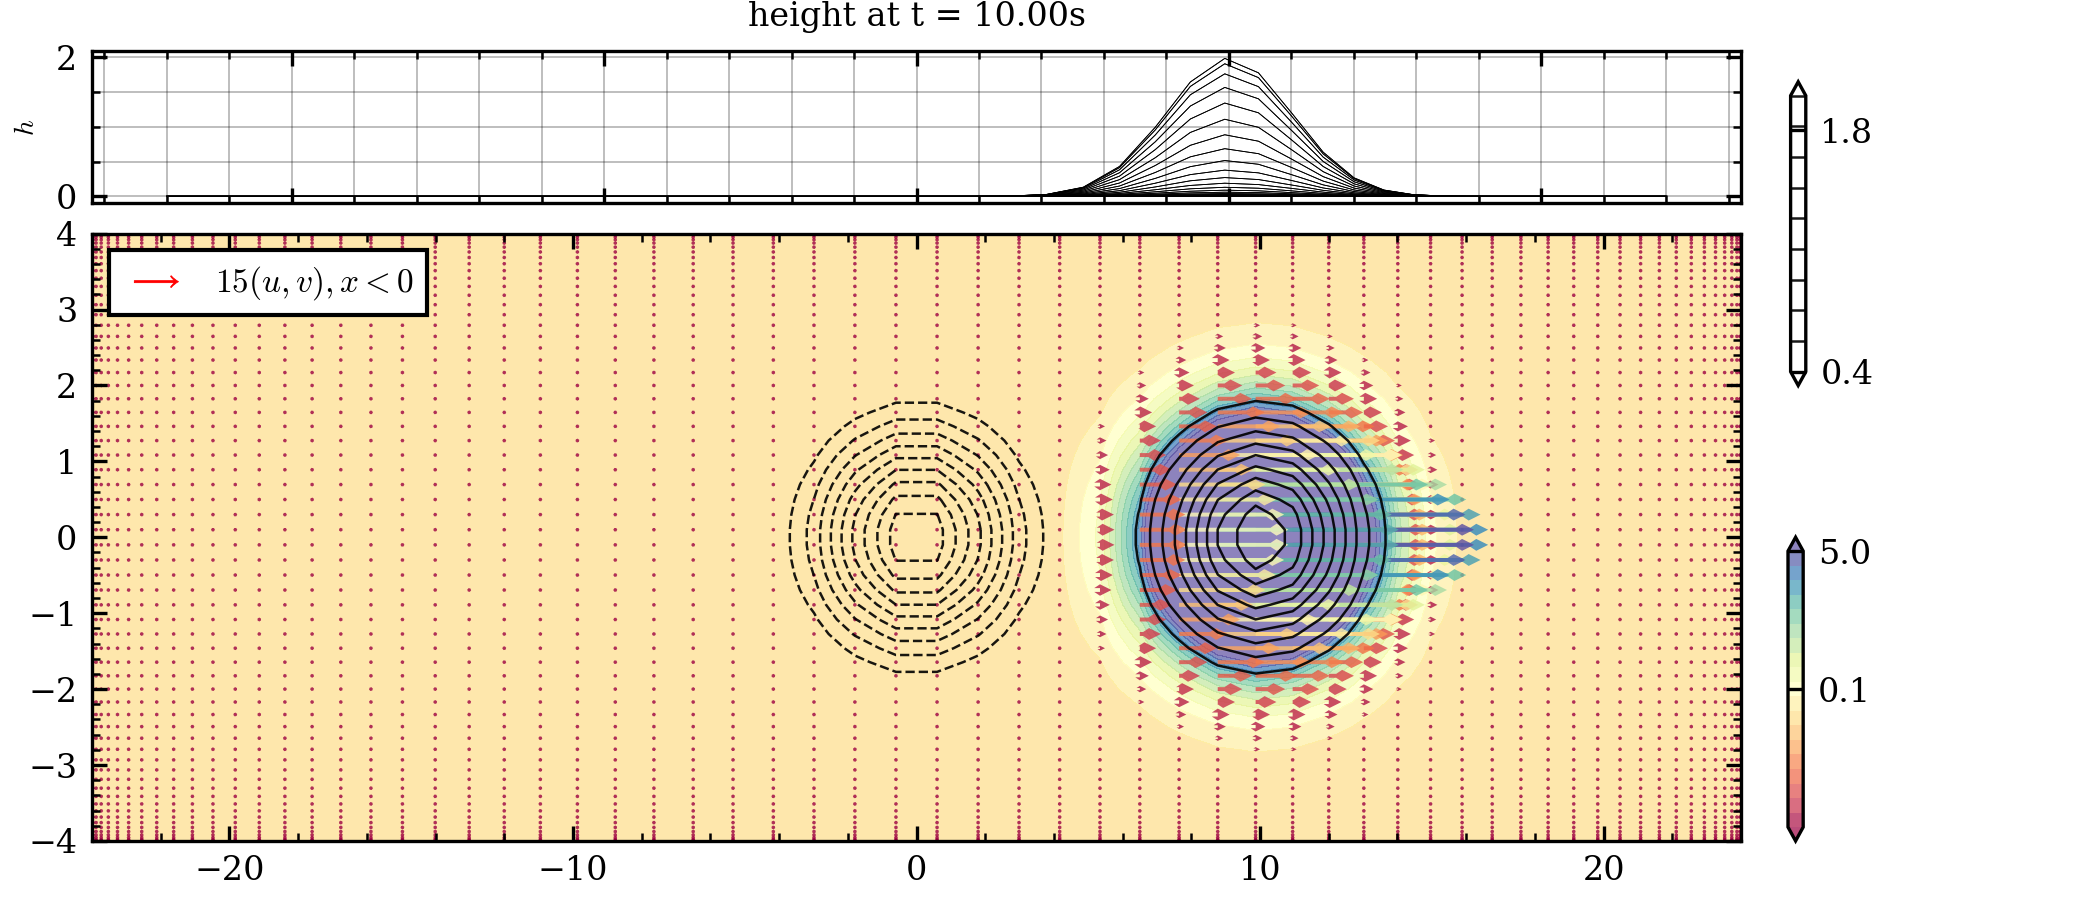
\includegraphics[width=\textwidth]{./figure/kelvin_wave.png}
\end{figure}
\captionof{figure}{The eastward propagating of the kelvin is clearly visible, the initial conditions are dashed plotted in black. Furthermore, we can notice through the velocity field study that the main specificity of the kelvin wave \textbf{$v = 0$} is verified. There are no dispersion or deformation effects of the soliton, which is reasonable since Kelvin waves are non-dispersive.
    This behavior is the result of a balance between the height gradient imposed by the Kelvin wave shape, and the Coriolis force. Indeed, in the northern-hemisphere the height gradient projected on the north south-north axis, which tends to spread the wave in the north direction is exactly compensate by the Coriolis force which acts in the east direction, hence we keep $V = 0$. This is exactly the same in the southern-hemisphere, but with the opposite direction. This explains why the Kelvin wave are propagating eastward, and cannot propagate westward.
    It highlights also the importance of the \textbf{spatial scale} of the wave to have sufficient effect of Coriolis force}
\begin{multicols}{2}

    \subsubsection{Conservation of mass \& energy}
    \begin{figure}[H]
        \centering
        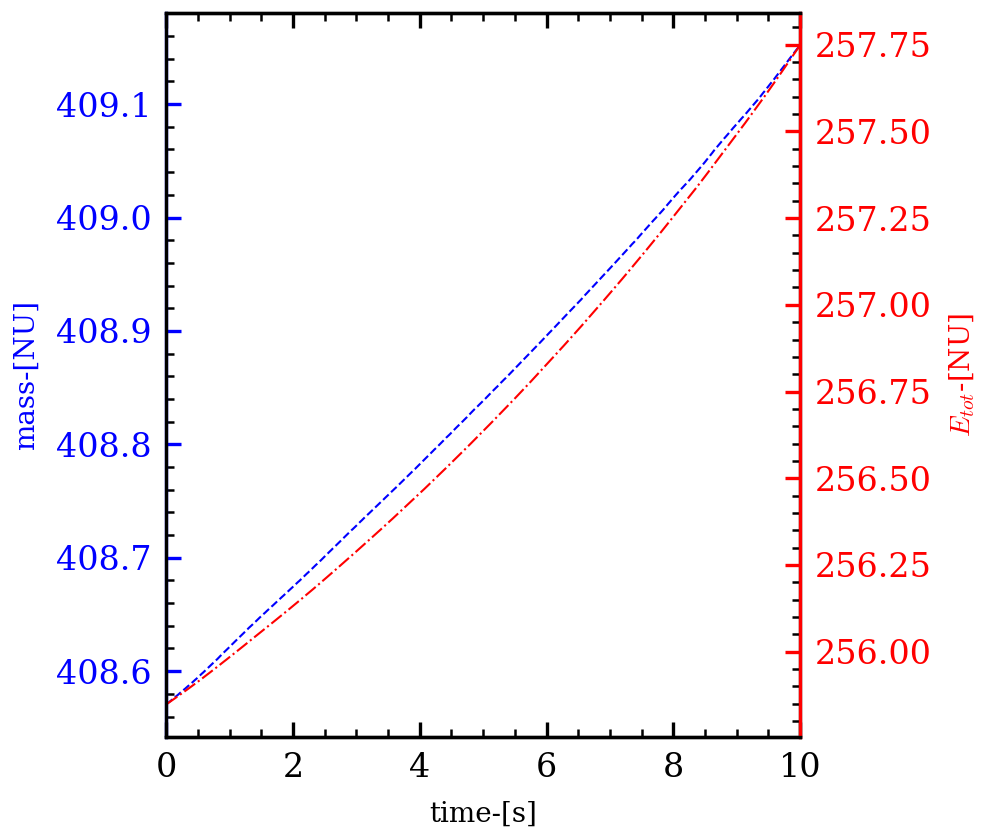
\includegraphics[width=\linewidth]{./figure/energy_kelvin_wave.png}
        \caption{The conservation of mass and energy are relatively good, the mass is conserved up to $2e^{-3}$, and the energy up to $4e^{-3}$, this is due to the numerical error, indeed there is no dissipation is our model. Note that the relative errors are greater than the one obtained for the Rossby soliton, this is due to the fact that the Kelvin wave is propagating much faster than the Rossby soliton, hence the numerical error is more important, The CFL condition are more restrictive, and taking the same time discretization as for the Rossby soliton is not the optimal method.}
        \label{}
    \end{figure}
    Considering the CFL condition :$$\Delta t \le  C_{max} N^{-2} \approx 1.8e^{-3}.$$ With the time step used we are quite close from the CLF condition, which is not the case for the Rossby soliton, this is why the numerical error is more important for the Kelvin wave.
    \subsubsection{Potential Vorticity}
    As the Rossby wave presents no south-north velocity component, the shedding of instabilities as it was the case for the Rossby soliton is not possible. Hence, the Potential Vorticity should remain constant with no oscillations, which were \textbf{characteristic of radiative instabilities}.

    \begin{figure}[H]
        \centering
        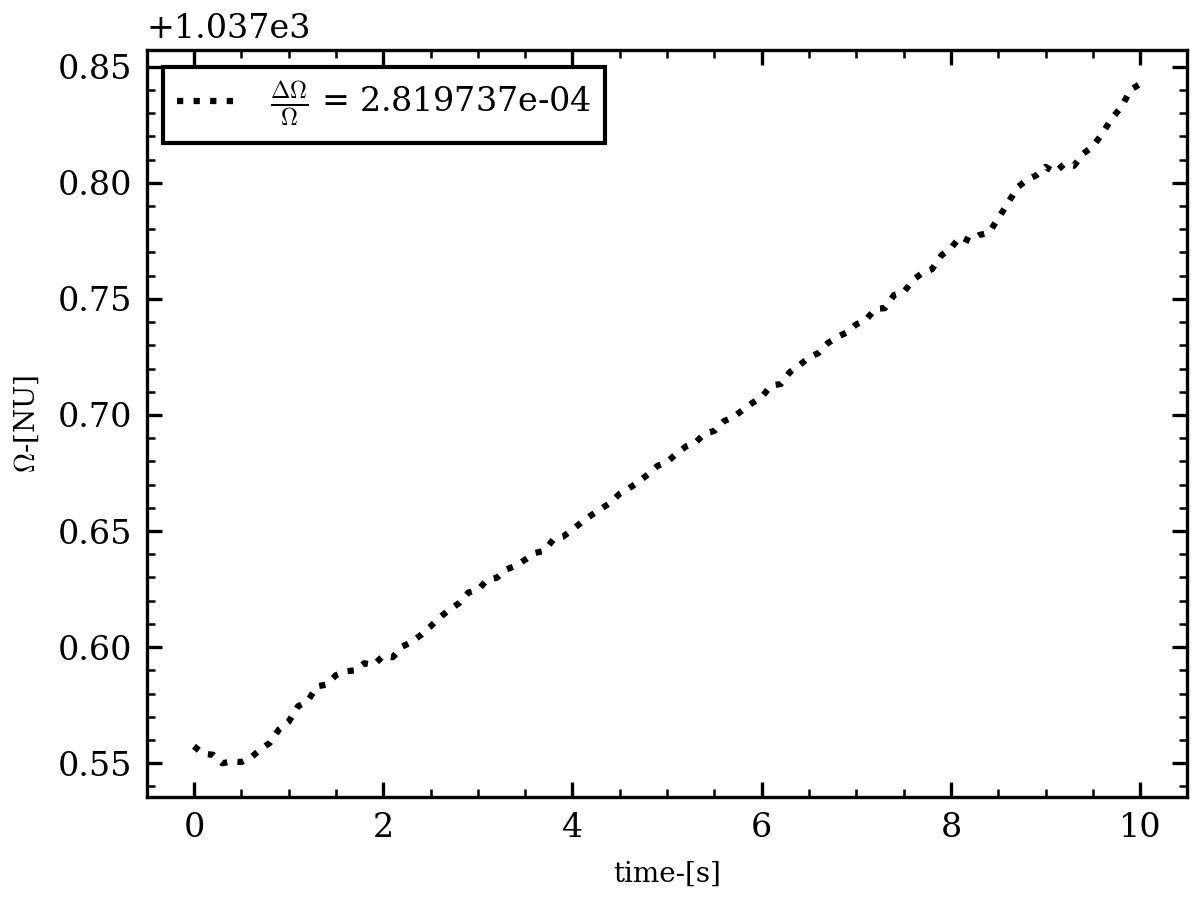
\includegraphics[width=1\linewidth]{./figure/potential_enstrophy_kelvin_wave.png}
        \caption{As intended, the potential vorticity remains quite constant with a relative error $\approx 2e^{-4}$. In addition to that no oscillations are visible in the enstrophy potential, which is a good indicator of the absence of radiative instabilities, as highlighted previously.}
        \label{}
    \end{figure}

    \subsubsection{Phase speed and dispersion }
    To evaluate the phase speed, we used a different method than the one used for the Rossby soliton (convergence issue), we fit the solution with a Kelvin wave shape, and for each time steps we track the dispersion and the position of the wave, this leads to the following :
    $$  h(x_0,y_0) = A \exp(-\tfrac{1}{2} ([k(x - x_0)] ^2 +[l(y - y_0)]^ 2)) $$
    The fit provides us the wave parameter $A, x_0, y_0, k, l$,:
    \begin{figure}[H]
        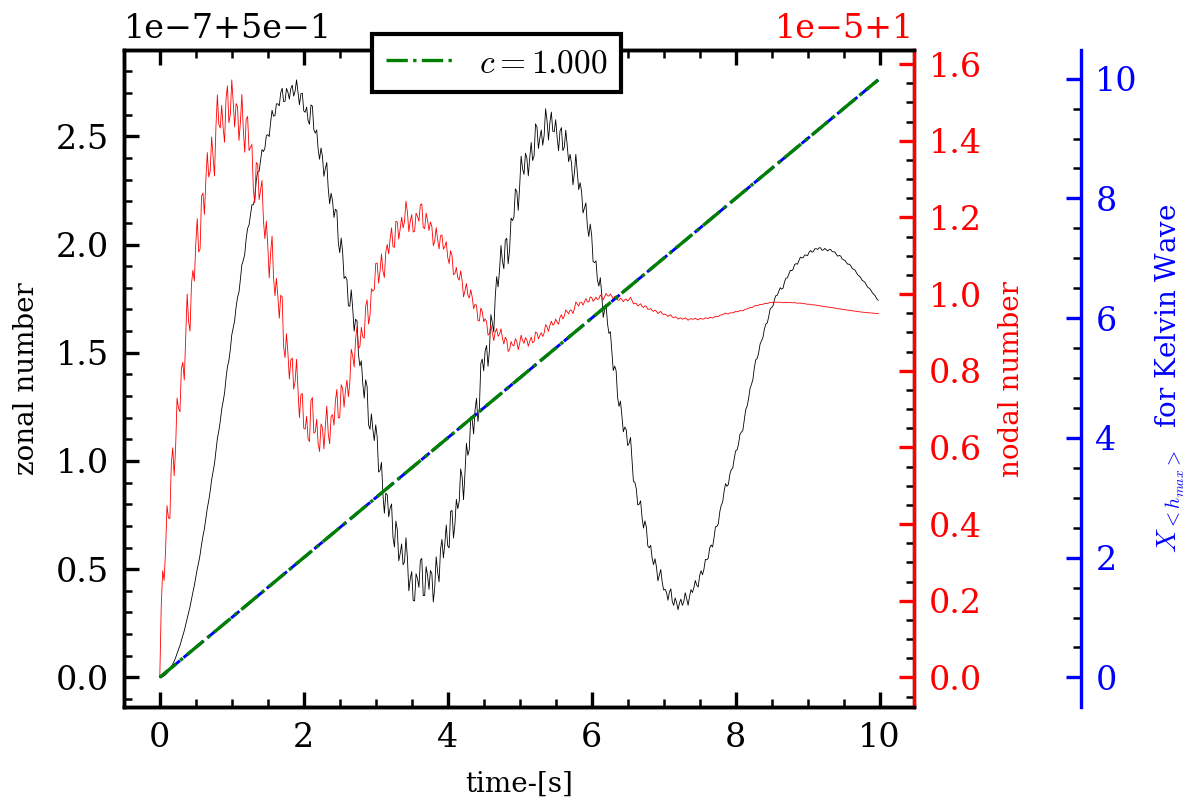
\includegraphics[width=1\linewidth]{./figure/kelvin_wave_param.png}
        \caption{The speed velocity is evaluated by tracking the position of the wave, and the dispersion is evaluated by tracking the amplitude of the wave. The phase speed calculated $c_\Phi^{\text{num}} = 1.000 = c_\Phi^{ana}$, which is the theoretical phase speed of the Kelvin wave.
            Regarding the dispersion, we have good results with a relative dispersion of $1e^{-5}$, for zonal and nodal wave number.}
    \end{figure}

    \subsection{Unstable waves}
    For simulating the behavior of unstable waves we used the following parameters :
    \begin{center}
        \begin{tabular}{ccccc}
            \toprule
            \multicolumn{5}{c}{characteristic scales}    \\
            \cmidrule{1 -5}
            $a_0$ & $\beta$ & $g$    & $N$  & $\Delta t$ \\
            \midrule
            $1$   & $1$     & $1$ ns & $64$ & $2e^{-3}$  \\
            \bottomrule
        \end{tabular}
    \end{center}
    We call unstable wave, wave that have no velocity field for initial condition, hence the gravity at the origin of motion the only force applied is the gravitational force, which tends to spread the wave in every direction. This is why we will take a wave with quite small nodal and zonal wave number to have a great influence of the Coriolis force on the motion.
    We will take a wave of the following form :
    \begin{equation}
        \label{eq:sharp wave}
        \begin{cases}
            h(x,y,t = 0) = H_0  \exp(- ((0.5x) ^2 +(y)^ 2)) \\
            u(x.y, t = 0) = 0                               \\
            v(x,y,t=0) = 0
        \end{cases}
    \end{equation}
    Which is a simple kelvin wave with no west-east velocity field. To simulate these waves we will take the following parameters :
    \begin{center}
        \begin{tabular}{c c c}
            \toprule
            \multicolumn{3}{c}{Parameter} \\
            \cmidrule{1 -3}
            $H_0$ & $k$   & $l$           \\
            \midrule
            $2$   & $0.5$ & $1$           \\
            \bottomrule
        \end{tabular}
    \end{center}
    Note that as the gravity is the only force applied at the beginning, the wave should spread equally in every direction, hence the \textbf{mass of fluid should be equally distributed} east-west.

\end{multicols}

\begin{figure}[H]
    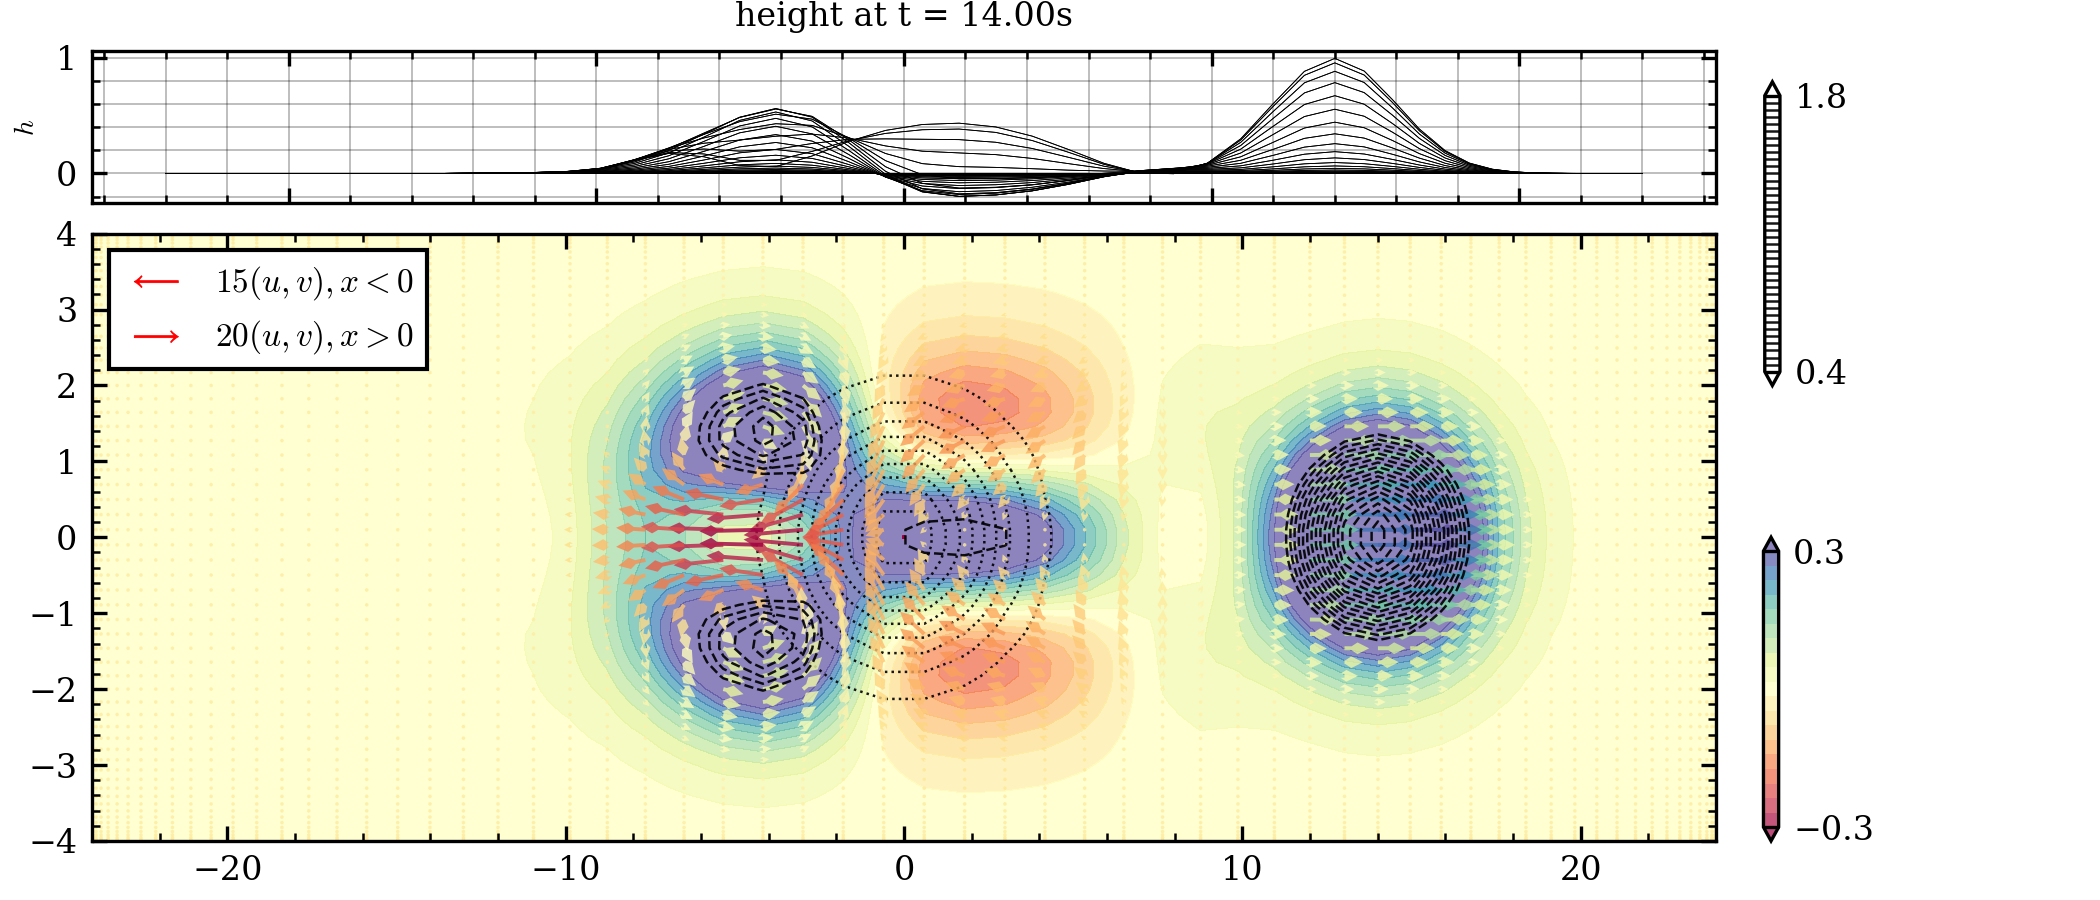
\includegraphics[width=\textwidth]{./figure/kelvin_wave_0_speed.png}
\end{figure}
Figure 2.12: Contour of the flow for $h\in[-.3,3]$ and $h\in[0.4,1.8]$ for the dashed contour lines. The original wave is split into two modes of propagation : one eastward the \textbf{Rossby soliton} $n = 1$ mode and one \textbf{Kelvin wave} mode. We can assert that  the westward propagating soliton has the same amplitude and phase speed, as the Rossby soliton $n = 1$ studied previously, the eastward propagating soliton matches the Kelvin wave phase speed and seems to have no dispersion. Furthermore, we have
$h = u$  with $V = 0$, which characterized the Kelvin wave Fig.2.8. \textbf{Radiative instabilities} are also present (here in the center of the flow), and presents the same behavior as the ones of the Rossby soliton. This splitting is majorly due to the initial conditions imposed.
The absence of east-west velocity introduces a gravitational spreading of the wave in every direction, and then an east-west velocity, which force the wave to split into an eastward wave(the Kelvin wave) and a westward wave (the Rossby soliton), let's note that if we took a wave with a bigger nodal number, the splitting would have been into gravitational waves, and not Kelvin | Rossby waves.
Finally, this splitting seems equally distributed in energy, as it will be discussed in the next section.

\begin{multicols}{2}
    \begin{figure}[H]
        \centering
        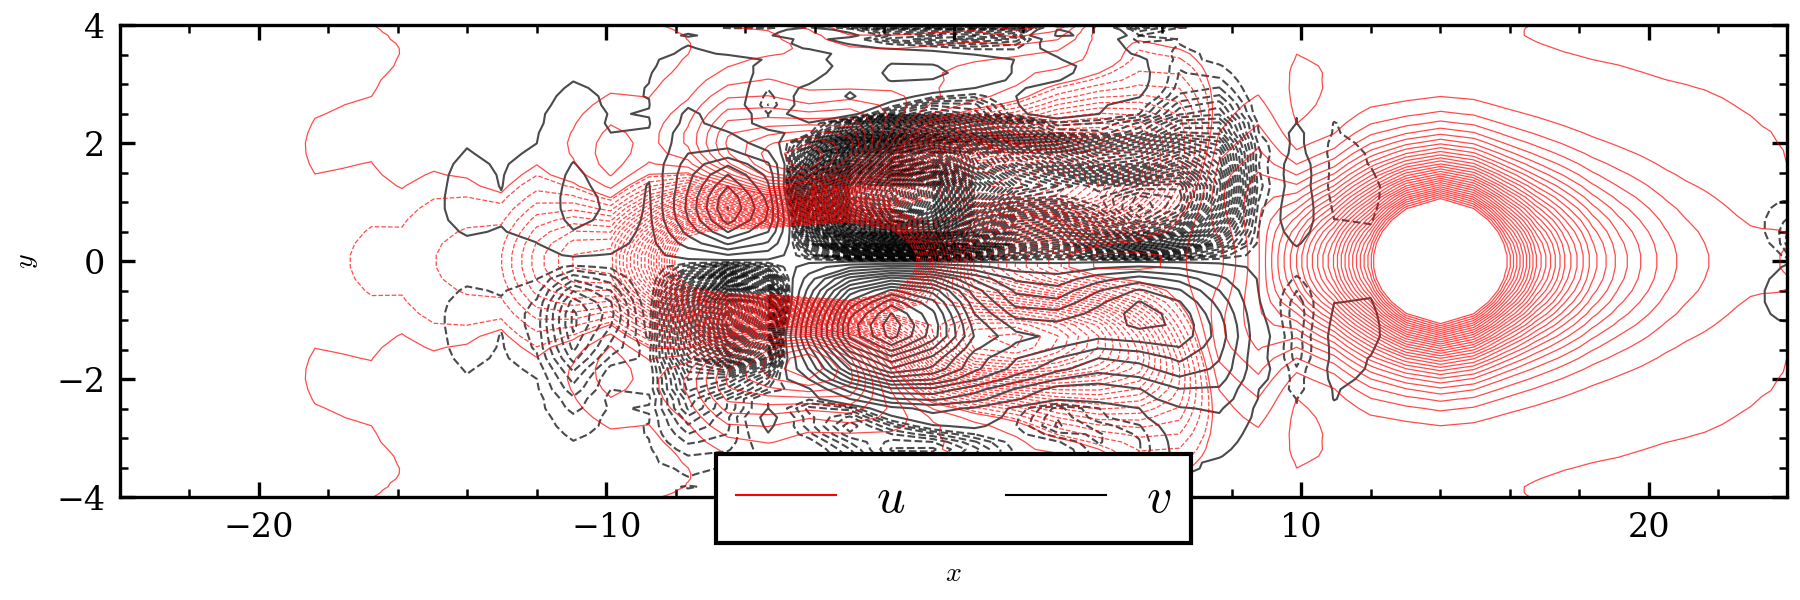
\includegraphics[width=1\linewidth]{./figure/velocity_common_wave.png}
        \caption{Here we can see that there is no hesitation regarding the type of the waves, indeed the eastward wave presents no south-north velocity component, furthermore the wave is satisfying all the Kelvin wave properties. Where,
            the westward wave presents instability nodations and a characteristic Rossby south-north velocity field Fig.\ref{fig:vfield Rossby}.}
        \label{}
    \end{figure}
    \addtocounter{figure}{+1}

    \subsubsection{Conservation of mass \& energy}
    The splitting into two east-west modes, raises the question of the energy repartition between the two modes, indeed the initial conditions are symmetric, and the only force applied is the gravitational force, which is symmetric as well. Hence the Volume and the mass should be equally distributed between the two modes.
    Lets's note that the Kelvin wave amplitude is two times smaller than the initial one. And note that for this type of Gaussian wave we have the following relation for the wave volume :
    $$V = 2 \pi H_0 kl$$
    Hence the volume of the Kelvin wave is two times smaller than the initial one, this leads to an equipartition in mass between both modes. This shows that the kinetic Energy $T$ is not equally distributed between the two modes, since the Kelvin wave is 3 times faster than the Rossby soliton. This leads to
    \begin{equation}
        T_{\text{Kelvin}} = 9 T_{\text{Rossby}}.
        \label{eq:T}
    \end{equation}



    \begin{wrapfigure}[20]{r}{0.4\linewidth}
        \hspace*{-0.2cm}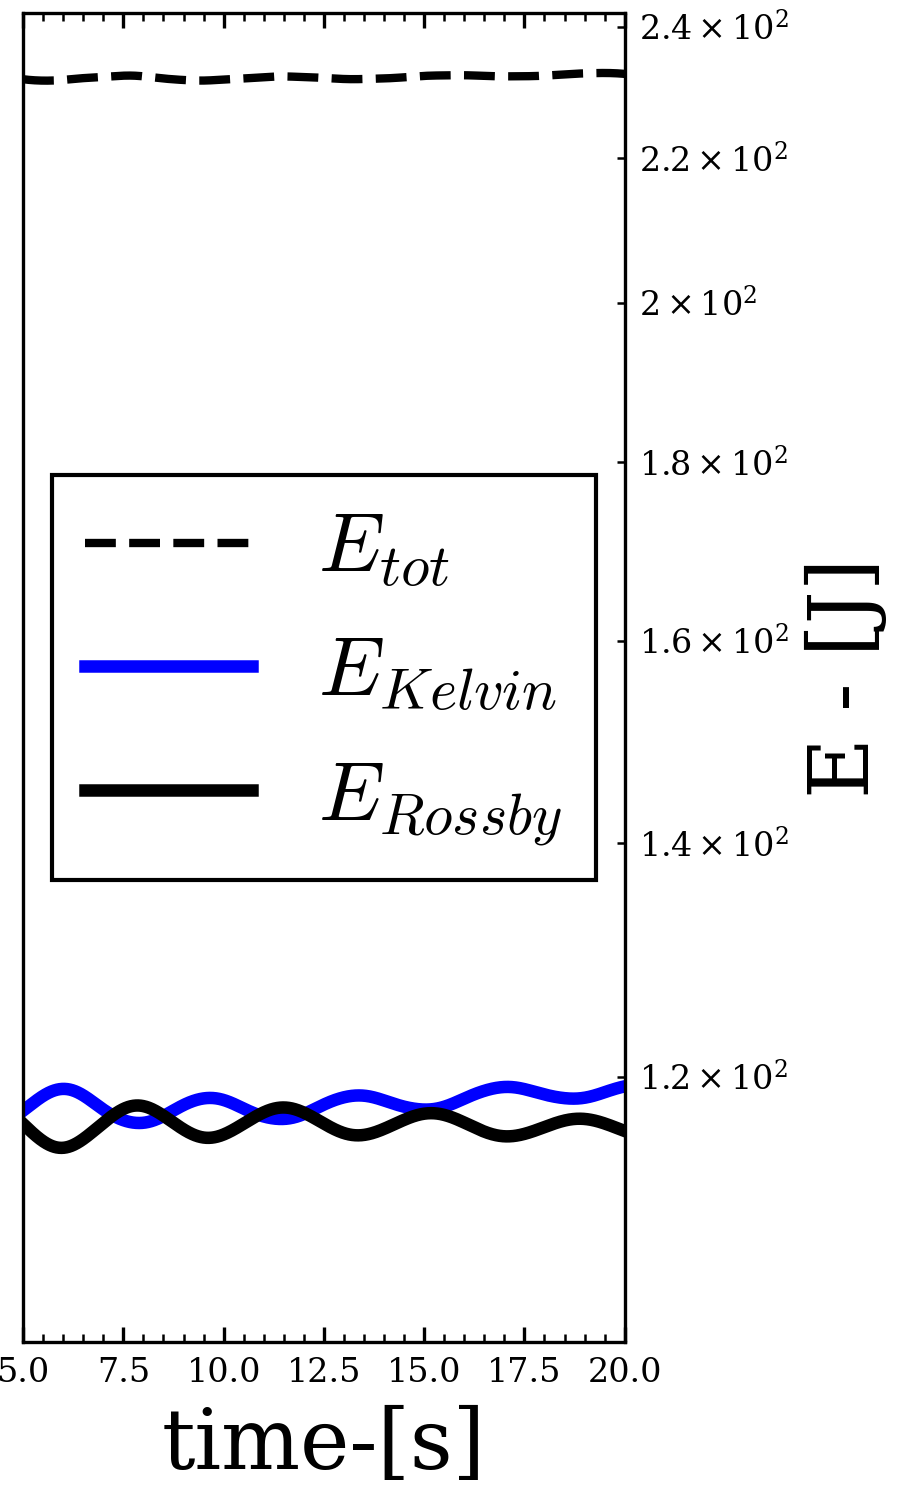
\includegraphics[width=1.2\linewidth]{./figure/energy_repartition.png}
    \end{wrapfigure}
    Figure 1.13 The following figure highlights very interesting behavior of the splitting. Firstly the global energy is equally distributed between the two modes, which leads to the conservative properties' \refeq{eq:T}, \refeq{eq:Epp}
    Indeed, the Rossby wave and the Kelvin wave have mostly the same total energy. However, the very small oscillations in the energy of these is waves is quite surprising.
    Indeed, both modes oscillate with perfectly $\pi / 2$ phase shifted. Every time the Rossby soliton reach a maximum of energy the Kelvin wave reaches a minimum, and vice versa. This is quite surprising, and can be explained by the following : the instabilities shed by the Rossby soliton are periodically reducing the soliton energy in the computation, while propagating eastward influencing the computation of Kelvin wave energy.
    Now let's evaluate the energy conservation of the global flow.
    \begin{figure}
        \caption{\phantom{a}}
    \end{figure}

    \begin{figure}[H]
        \centering
        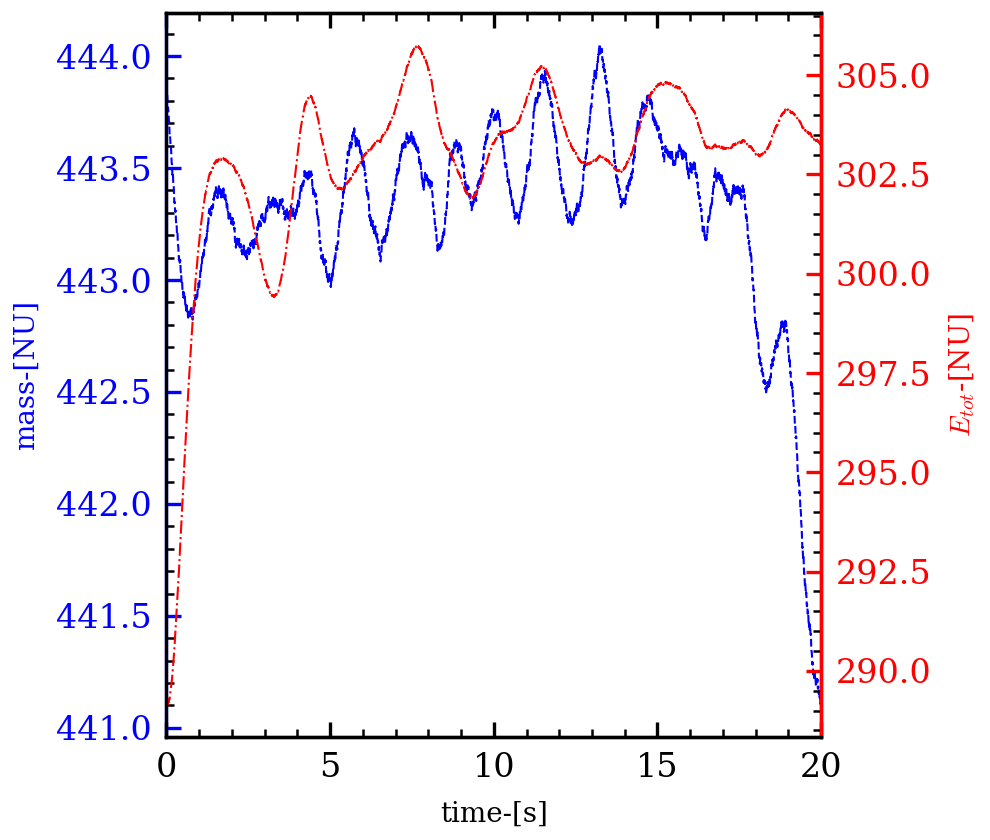
\includegraphics[width=\linewidth]{./figure/energy_common_wave.png}
    \end{figure}
    \captionof{figure}{The conservation of mass and energy are quite good, the relative difference in mass and energy is up to $6e^{-3}$. Furthermore,
        it seems to have no dissipation as opposed to the Rossby | Kelvin case, one idea to explain this is that as seen previously the Kelvin wave gains energy over time as opposed to the Rossby waves, hence these two numerical errors may compensate each other.
        Finally, the oscillations in energy and mass seems to correlated with the radiative instabilities shed by the Rossby soliton.}

    \subsubsection{Potential Vorticity}
    \phantom{doisa}
    \begin{figure}[H]
        \centering
        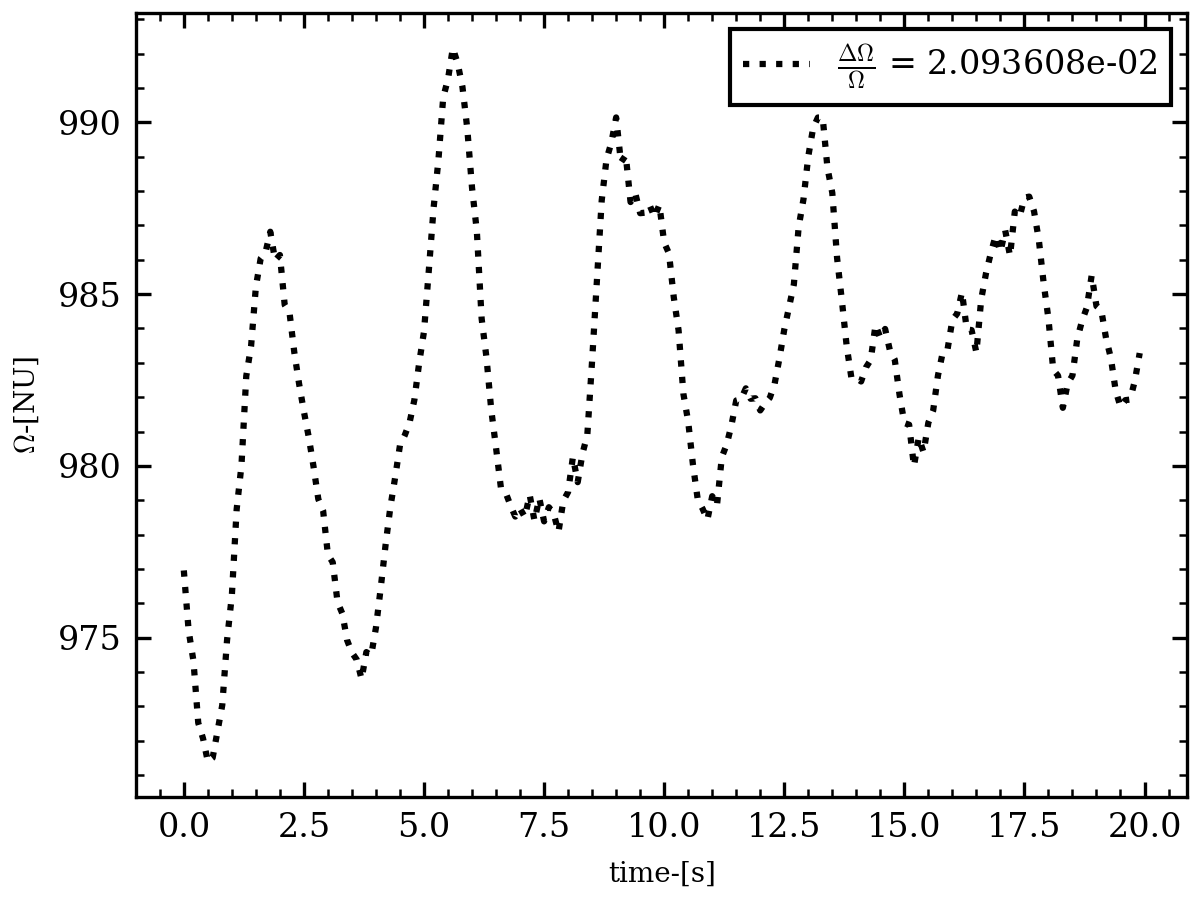
\includegraphics[width=1\linewidth]{./figure/potential_enstrophy_common_wave.png}
        \caption{The relative difference in potential enstrophy here is about $2e^{-2}$ this relatively low metrics and the strong oscillations can be explained respectively by the CLF conditions and the radiative process of instabilities}.
        \label{}
    \end{figure}
    \subsubsection{Phase speed and dispersion evaluation}
    To study the phase speed and the dispersion of the Kelvin wave we used the same method as for the previous part, fitting the Kelvin wave with the appropriate wave shape. This leads to the following :
    \begin{figure}[H]
        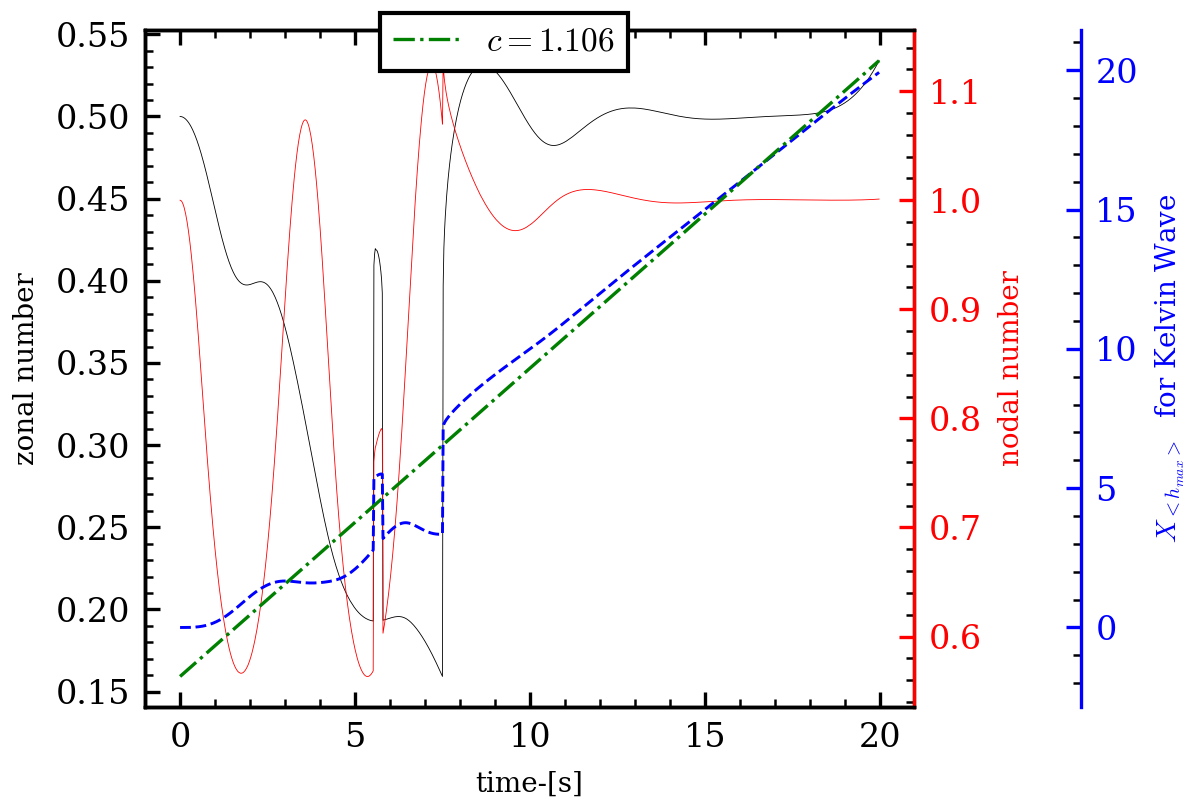
\includegraphics[width=1\linewidth]{./figure/0velocity_wave_params.png}
        \caption{\textbf{Phase speeds evaluation and dispersion for the Kelvin wave} : we got $c_\Phi^{\text{num}} = 1.106$. This gives $C_{num}/C_{ana} = 1.106$ Regarding the dissipation, we have good result indeed, when the splitting is finished at $t = 10s$ we got a near constant nodal and zonal wave number equal to the initial one, which is very interesting because only the height of the Kelvin wave have changed.}
    \end{figure}
    For the Kelvin wave the dispersion \& amplitudes studies lead to the following equation for the Kelvin mode :
    \begin{equation}
        \label{eq:num approx}
        \begin{cases}
            h(x,y,t) = \exp{(-\tfrac{1}{2}([0.5(x -t)]^2 + 1y^2))} \\
            u(x,y,t) = h(x,y,t)                                    \\
            v(x,y,t) = 0
        \end{cases}
    \end{equation}
    \begin{figure}[H]
        \includegraphics[width=1\linewidth]{./figure/0velocity_wave_params_Rossby.png}
        \caption{\textbf{Phase speeds evaluation and dispersion for the Rossby wave}: we got $c_\Phi^{\text{num}} = -0.304 $. This gives $C_{num}/C_{ana} = 1.03$. For the Rossby wave the dissipation study presents a very interesting behavior, the Hermite coefficients  eq.\refeq{eq:6} are oscillating around a steady states (horizontal line in red for $H_2$ coefficient and in black for $H_0$ coefficient)
        . This is mostly due to instabilities shedding, these oscillations stands for a variation in the ratio : $k/\sigma$ with a wave deformation when a instability is shaded.
        However, at steady state the ratio of the Hermite polynomials coefficients is constant, satisfying the Rossby soliton equation \refeq{eq:Rossby}.}
    \end{figure}
    For the Rossby wave the dispersion study leads to the following equation for the $n = 1$ mode :
    \begin{equation}
        \label{eq:num approx}
        \eta(\xi, \tau) = 4.589 \text{sech}^2[B(\xi - 0.395B^2\tau)]
    \end{equation}


    With exactly the same coefficients as the one obtained by Boyd \ref{eq:Rossby} for the Rossby soliton (respectively $\tfrac{3}{4}$ and $\tfrac{3}{2}$ for $H_0$ and $H_2$), with the same zonal wave number $B = 0.395$.

    \begin{equation}
        \label{eq:num approx}
        \begin{cases}
            h(x,y,t) = \eta(x,y) \frac{3 + 6y^2}{4}\exp(-\tfrac{1}{2}y^2)  \\
            u(x,y,t) = \eta(x,y) \frac{-9 + 6y^2}{4}\exp(-\tfrac{1}{2}y^2) \\
            v(x,y,t) = -2yB\eta(x,y) \tanh(Bx)\exp(-\tfrac{1}{2}y^2)
        \end{cases}
    \end{equation}

    \chapter{Summery \& Prospectus}

    In conclusion, the numerical simulations employing a Chebyshev spectral method on a non-normalized domain, combined with a second-order accurate leap-frog-like time discretization, proved effective in studying the dynamics of Poincaré waves. The simulations encompassed various wave scenarios, revealing noteworthy behaviors. For the Rossby soliton, the observed westward propagation and minimal damping align with anticipated characteristics, despite minor numerical errors. The analysis of the CFL condition and the application of a boundary condition contributed to the scheme's robustness. Conservation of mass and energy remained crucial for evaluating the numerical efficiency.
    The study of Kelvin waves showcased their non-dispersive nature, exhibiting eastward propagation without deformation or dispersion. Conservation of mass, energy, and constant potential vorticity underscored the accuracy of the numerical scheme.
    Unstable wave simulations elucidated the equal distribution of energy between Rossby and Kelvin modes, demonstrating a conservative behavior. The observed ninefold difference in kinetic energy between the Kelvin wave and the Rossby soliton provided valuable insights into energy partitioning dynamics.
    In summary, the numerical integration scheme, characterized by its spatial discretization strategy and time-stepping approach, successfully captured the essential features of Poincaré waves. The findings contribute to the understanding of wave dynamics, numerical methodologies, and the intricate interplay between different wave modes within the context of shallow water equations.

    Finest analysis on other wave types would be interesting to study, specially for the mode splitting and the energy repartition between modes. For example, we could have unearthed higher Rossby mode by studying bigger scale waves, with a stronger mesh refinement. The use of \emph{Sponge Layer} to limit computation costs,
    would have been interesting to study as well. Some interrogations remain about the difference in oscillation frequency between the mass and the energy for the Rossby wave. Furthermore, the theoretical explanation of the instabilities shedding is not perfectly clear for the $n = 1$ modes.

\end{multicols}
\printbibliography
\end{document}